
\documentclass[letterpaper,twocolumn,10pt]{article}
\usepackage{Fast/usenix-2020-09}


\usepackage{amsmath}
\usepackage{amsfonts}
\usepackage{amssymb}
\usepackage{booktabs}
\usepackage{stmaryrd}
\usepackage{graphicx}
\usepackage{listings}
\usepackage{pgfplots}
\usepgfplotslibrary{groupplots}
\usepackage{pgfplotstable}
\usepgfplotslibrary{fillbetween}
\usepackage{subcaption}
\pgfplotsset{compat=1.18}
\usetikzlibrary{positioning}
\usepackage[scaled=.8]{beramono}
\usepackage{svg}
\usepackage{caption}
\usepackage{subcaption}
\usepackage{syntax}
\usepackage{textgreek} % for \textDelta
\usepackage{comment}
\usepackage{verbatim}
\usepackage{url}

\title{Using Static Analysis of Python Programs for Efficient Checkpointing}
\author{}
\date{August 2025}

\begin{document}

\maketitle

\begin{abstract}
Static analysis of Python programs faces significant challenges due to dynamic typing, reflection, and flexible control structures. However, important classes of Python programs --- particularly in numerical computing --- often avoid these problematic features, using explicit type annotations and predictable control flow patterns that may enable effective static reasoning.

We demonstrate that standard program analysis techniques can be successfully applied to well-structured Python programs to enable practical optimizations. Our approach combines points-to analysis, type inference, and liveness analysis, augmented with lightweight effect annotations for built-in types and external libraries. To demonstrate the framework's utility, we develop a specialization that performs escape analysis across loop iteration boundaries, automatically identifying minimal persistent state for iterative algorithms.

We apply this analysis to synthesize selective checkpointing instrumentation for realistic numerical Python programs, including k-means clustering, orthogonal matching pursuit, and graph search algorithms. Our evaluation shows that this approach can achieve checkpoint size reductions of 2--5 orders of magnitude compared to system-level alternatives, demonstrating that established static analysis techniques --- when carefully applied to structurally constrained Python code --- can enable significant automated optimizations.

% Systems:
% Checkpointing is a critical mechanism for fault tolerance in distributed computing systems. However, traditional system-level approaches --- such as full-process or VM state capture --- introduce significant overhead by indiscriminately storing entire memory snapshots. Application-aware checkpointing addresses this by selectively preserving only semantically relevant state, but such techniques have seen limited adoption in dynamic languages like Python due to the challenges of static analysis.

% We show that for a some classical machine learning algorithms implemented with NumPy and SciPy, application-aware checkpointing is both feasible and highly effective. Our approach leverages abstract interpretation to combine type inference, points-to analysis, and liveness analysis, identifying the minimal set of variables required to safely resume execution after failure.

% We implement this technique and evaluate it on several non-trivial Python ML workloads. Compared to system-level tools like CRIU~\cite{venkatesh2019fast} and naive checkpointing strategies that preserve all local state, our method reduces checkpoint size by 2--5 orders of magnitude. This makes frequent, low-overhead checkpointing practical in environments where traditional methods are otherwise prohibitive.

% Synchronization of replicated data and program state is an essential aspect of application fault-tolerance. 
% It allows quick recovery when a crash occurs on a
% compute node, reducing downtime and data loss.
% Current solutions use virtual memory mapping to identify page writes and replicate them at the destination. This approach has its limitations because the granularity is restricted to a minimum of 4KiB per page, which may result in more data being replicated. 
% Motivated by the emerging CXL hardware, in a recent work Waddington, et al. [SoCC 22] demonstrated that using compression algorithms on VM snapshot data at cache line granularity may significantly improve the size of the replicated data to be synchronized. 

% In this work we use static analysis techniques to analyze the execution of programs and store a succinct space that represent the execution state within in a loop. We automatically identify the variables that need to be stored for fault-tolerance, so that if the software crashes we can resume given that data. We demonstrate that using these static analysis techniques on several popular machine learning algorithms, we are able to identify and synchronize much more succinct data (about two orders of magnitude) compared Waddington, et al. [SoCC 22].
\end{abstract}


\section{Introduction}
Python powers much of modern numerical computing through libraries like NumPy. The language’s dynamic features, such as dynamic typing, reflection, and flexible control flow, make static analysis notoriously difficult. Yet many Python programs deliberately avoid these constructs, favoring typed, deterministic code and stable libraries. For such well-structured code, we show that established static analysis techniques can be usefully adapted to specific domains of interest. We focus on one important problem domain: efficient checkpointing of long-running programs. 
In this work we demonstrate leveraging static analysis information to perform light-weight instrumentation, reducing storage writes by orders of magnitude compared to existing checkpointing approaches.

Checkpointing is the task of capturing the program’s state at designated points to enable recovery of work done after failure. Unexpected faults in long-running or resource-intensive computations can lead to costly recomputation and lost work. Traditional checkpointing is typically implemented at the system level, treating applications as black boxes. Tools, such as CRIU~\cite{CRIUProject}, snapshot the entire Linux process, including memory, file descriptors, and registers. Virtual machine snapshots~\cite{VMwareSnapshot, RedHatVMSnapshot} go further, capturing entire guest operating system state. While robust and language-agnostic, this approach is usually highly inefficient as it demands large amounts of data be written to storage --- even when done incrementally.

Application-level checkpointing offers an alternative: preserving only the program state that influences future computation. A naive approach might be capturing all reachable state from within the scope of the current program location. Capturing all reachable state is overly conservative. Much of the state is immutable or transient and not needed after resumption.  This naive approach might result in even worse performance than checkpointing the entire process incrementally.

% A more sophisticated approach is to look for the specific parts of program state that are both mutated and required for resumption of the computation. This idea dates back decades~\cite{li1990catch} and has recently resurfaced~\cite{kim2024lact}. However, it has seen virtually no adoption in dynamic languages such as Python. The difficulty lies in the language’s dynamic semantics --- runtime typing, reflection, closures --- that make sound static analysis difficult.

Prior work has shown that analysis-assisted checkpointing can shrink state substantially by saving only data that remain live across a restart. This idea dates back to CATCH~\cite{li1990catch} and to application-level frameworks in HPC such as C3 and CPPC, which use program analysis to identify variables that will be read after a checkpoint and to instrument code accordingly ~\cite{bronevetsky2004application,rodriguez2010cppc}. Recent work revives this direction, computing liveness over array slices to exclude dead values and reduce writes~\cite{kim2024lact}. To our knowledge, comparable liveness-based minimization has not been attempted for fully dynamic languages like Python; dynamic typing, reflection, and mutable object layouts complicate sound, precise liveness and pointer analysis.

That said, many Python workloads already operate within a restricted, well-structured subset of the language~\cite{bence2021unambiguity}. They avoid reflection, rely on type annotations, follow predictable control flow, and depend on stable libraries with well-understood semantics. While these practices limit some of Python’s flexibility, they are common in scientific computing, where correctness and performance outweigh dynamic features. Use of this subset of language features defines the class of programs our static analysis targets.

Our framework combines liveness, pointer, and type analyses with lightweight effect annotations. These annotations classify operations in built-in types and external libraries as allocating, mutating, or pure, enabling analysis of third-party code while maintaining useful precision in heap-shape tracking. In contrast to traditional ``defensive'' analyses, we adopt a \emph{happy-path} approach: assuming the program is correct and inputs are valid, in order to focus precision on the intended execution path.

Building on this framework, we introduce an analysis that identifies the \emph{minimal persistent state}—the subset of program state that must be carried across iterations to ensure correct recovery. This analysis tracks heap shape over loop iterations, determines dirty state via pointer reachability, and restricts results to live variables. From this information we synthesize selective checkpointing logic that preserves only the semantically necessary state.

We evaluate the approach on realistic implementations of numerical algorithms: k-means clustering, orthogonal matching pursuit (OMP), and graph search procedures. These case studies confirm that static analysis techniques, carefully applied to structurally disciplined Python code, can yield major practical benefits.


\paragraph{Contributions}
\begin{enumerate}
\item A reusable static analysis framework for well-typed, structured Python code satisfying certain structural assumptions.
\item Specialized analysis and synthesis steps for checkpoint IO minimization via minimal persistent state analysis.
\item An empirical demonstration showing that semantically guided checkpointing is feasible and highly effective in practical, albeit constrained, Python workloads.
\end{enumerate}

The remainder of the paper is organized as follows. In \autoref{sec:running-example} we present a running example based on the K-Means clustering algorithm to illustrate the challenges and opportunities for selective checkpointing in numerical Python code. \autoref{sec:analysis} describes our analysis framework in detail, including the intermediate representation, the design of the type and pointer domains, and the interaction between liveness, type, and heap analyses. \autoref{sec:evaluation} evaluates our approach on several realistic workloads, comparing our synthesized checkpoints against naive and system-level baselines. \autoref{sec:related} discusses related work in static analysis for dynamic languages and checkpointing. We conclude in \autoref{sec:conclusion} with a summary of our contributions and directions for future work.


\begin{figure}[t]
\begin{lstlisting}[language=python]
import numpy as np

def kmeans(X:np.ndarray, k:int, iters:int)->np.ndarray:
    # initilization
    centroids = X[np.random.choice(X.shape[0], k)]
    clusters = list[list[int]]()
    for i in range(iters):  # type: int
        # loop body
        clusters = [list[int]() for _ in range(k)]
        for sample_i in range(len(X)):
            v = X[sample_i] - centroids
            r = np.linalg.norm(v, None, 1).argmin()
            clusters[r].append(sample_i)
        new_centroids = np.array([X[cluster].mean(0)
                             for cluster in clusters])
        if np.allclose(centroids, new_centroids):
            break
        centroids = new_centroids
    # finalization
    return compute_labels(clusters, X.shape[0])
\end{lstlisting}
\caption{\label{lst:code-kmeans}
K-Means clustering with $k$ clusters.}
\end{figure}

\section{Running Example: K-Means Clustering}
\label{sec:running-example}

We illustrate our checkpointing approach using the classical \emph{K-Means clustering} algorithm. This widely used iterative method partitions a dataset into $k$ clusters by repeatedly reassigning points to the nearest centroid and updating centroids as the mean of their assigned points.

Each iteration proceeds as follows:
\begin{enumerate}
    \item \textbf{Cluster assignment:} Each data point is assigned to its nearest centroid.
    \item \textbf{Centroid update:} New centroids are computed as the mean of each cluster.
    \item \textbf{Convergence check:} If centroids have not significantly changed, the algorithm halts.
\end{enumerate}

This style of computation is a natural fit for checkpointing: each iteration overwrites the previous cluster assignments and recomputes temporary data structures from scratch. Only the \texttt{centroids} array must persist across iterations. However, conventional checkpointing tools like CRIU or VM-based snapshots indiscriminately capture the full resident memory---including all temporary arrays and internal buffers---leading to high storage and I/O overhead.

Our system avoids this inefficiency by identifying the \emph{minimal} state necessary to resume execution after a crash. It does so through a static analysis pipeline that combines:
\begin{itemize}
    \item \textbf{Liveness analysis} to determine which variables are needed for future execution.
    \item \textbf{Points-to analysis} to track object references and heap structure.
    \item \textbf{Dirty analysis} to identify memory locations that were actually modified.
\end{itemize}
Applied to K-Means, the analysis concludes that only the centroid array is both live and dirty at the loop head. All other objects---including the \texttt{clusters} data structure, distance computations, and scratch space---are either recomputed or dead.

We automatically inject a checkpoint at the loop header using a lightweight transactional API:
\begin{lstlisting}[language=python]
# initilization unchanged
with Loader(__file__, locals()) as transaction:
    if transaction:
        [centroids] = transaction.move()
    for i in transaction.iterate(range(iters)):
        # Loop body unchanged
        transaction.commit(centroids)
# finalization unchanged
\end{lstlisting}
This enables recovery after a crash by restoring execution to the loop head with the correct value of \texttt{i} and \texttt{centroids}, without persisting irrelevant data. It is technically possible to make the instrumentation less syntactically intrusive, but the intention is to make it clear to the developer what the instrumentation does.

\paragraph{Language Features and Implementation Twists}

Although K-Means is conceptually simple, its Python implementation highlights several challenges for static analysis in a dynamic language. In particular:
\begin{itemize}
    \item \textbf{Generic data structures.} The variable \texttt{clusters} is a list of lists of integers. In order to enable type-checking and proper tracking of its structure, we require the use of explicit type constructors such as \texttt{list[int]()}. This ensures that our analysis can infer a meaningful and consistent type.
    \item \textbf{Side effects.} Function calls such as \texttt{xs.append(y)} mutate nested list. Our dirty analysis correctly tracks such effects to determine whether the object needs to be persisted. However, in this case, \texttt{clusters} is reconstructed every iteration and does not need to be saved.
    \item \textbf{Effect annotations.} For functions like \texttt{np.array} and \texttt{np.linalg.norm}, we rely on an internal library of effect annotations that describe whether a function allocates a new object, updates its arguments, or returns an alias. For example, \texttt{np.array} is treated as a constructor (``new''), while \texttt{np.mean} is considered pure. These annotations are essential for tracking heap mutations and avoiding conservative overapproximation.
    \item \textbf{Control-flow simplification.} Because Python bytecode is complex, we translate it to a simplified intermediate representation for verification and analysis.
\end{itemize}

Despite the simplicity of the target algorithm, precise analysis demands careful handling of Python's typing and memory model. Our implementation supports this through a combination of expressiveness in the type domain and selective annotation of external APIs. The result is an end-to-end system that enables lightweight, high-frequency checkpointing with no manual specification of which variables to save.

\section{Analysis}
\label{sec:analysis}

Our framework performs precise static analysis of Python programs within a tractable subset tailored to numerical computing. This enables advanced source-level transformations such as minimal checkpointing, demonstrated here as our main case study.

\subsection{Scope and Assumptions}
\label{sec:scope}

Our framework targets a practical subset of Python programs, chosen to balance analytical precision with tractable implementation.  
We disallow dynamic code evaluation, require statically resolvable function calls, mandate explicit instantiation for generics, and adopt a simplified aliasing model for NumPy arrays.  
These constraints, common in idiomatic numerical code, allow us to model control flow, data flow, and heap mutation soundly.

Several trade-offs shape the design: we abstract away array shapes, use a wildcard field for unknown collection elements, and leverage literal and variadic generics for precise yet extensible typing.  
Soundness depends on accurate type and effect annotations for external library calls.  

A full statement of these assumptions, including justification and implications, is given in Appendix~\ref{appendix:assumptions}.

\subsection{Intermediate Representation}
Our first step is to lower CPython bytecode to a \emph{register-based three-address code (TAC) intermediate representation} (Appendix~\ref{appendix:ir}), making data flow explicit. For example:
\begin{lstlisting}[language=Python]
# Python
x = f(y) + g(z)

# TAC
$1 = f(y)
$2 = g(z)
x  = $1 + $2
\end{lstlisting}
This removes implicit stack effects, ensures every instruction has explicit inputs and outputs, and simplifies dataflow reasoning.

\subsection{Overview of the Analysis Framework}

Our static analysis framework is built upon three core analyses: Liveness Analysis, Type Analysis, and Pointer and Dirty Analysis. These operate collaboratively within a \emph{reduced product domain}, meaning the insights from each analysis continuously inform and refine the others. This iterative refinement is crucial for overcoming the inherent imprecision that would arise if these analyses were run in isolation, allowing us to achieve a highly precise understanding of Python program behavior. The overall pipeline is visualized in Figure~\ref{fig:overview}.

\begin{figure}[t]
    \centering
    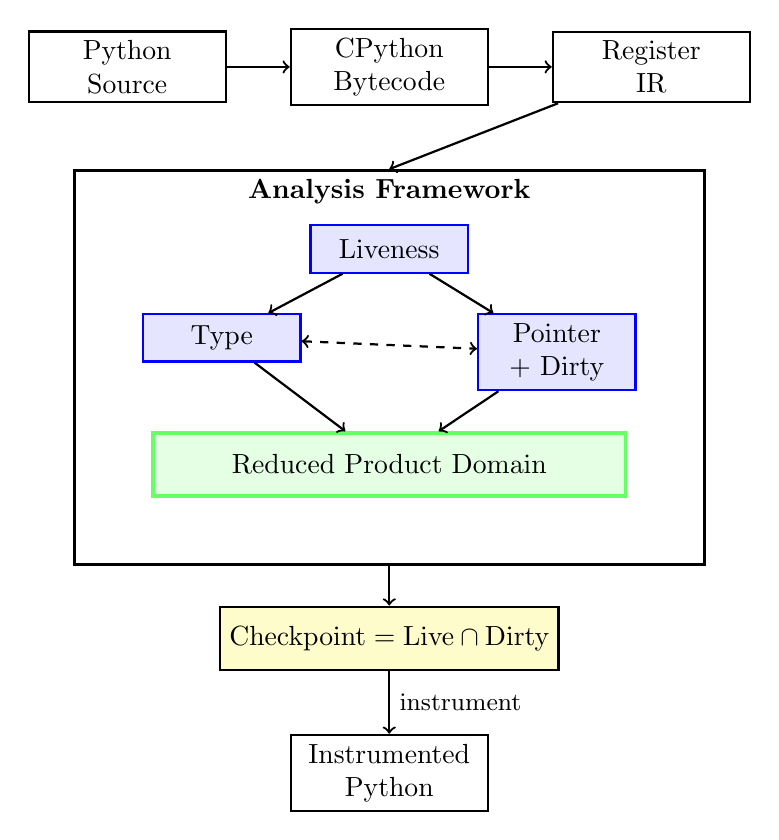
\begin{tikzpicture}[
    box/.style={rectangle, draw=black, thick, minimum width=2.5cm, minimum height=0.8cm, align=center},
    analysis/.style={rectangle, draw=blue, thick, minimum width=2cm, minimum height=0.6cm, align=center, fill=blue!10},
    arrow/.style={->, thick},
    darrow/.style={<->, thick, dashed},
    node distance=0.8cm
]

% Pipeline stages
\node[box] (source) {Python\\Source};
\node[box, right=of source] (bytecode) {CPython\\Bytecode};
\node[box, right=of bytecode] (ir) {Register\\IR};

% Analysis framework box
\node[rectangle, draw=black, very thick, minimum width=8cm, minimum height=5cm, below=0.8cm of bytecode] (framework) {};
\node[below] at (framework.north) {\textbf{Analysis Framework}};

% Three analyses inside framework
\node[analysis, below=1.5cm of bytecode] (liveness) {Liveness};
\node[analysis, below left=0.5cm and 0.1cm of liveness] (type) {Type};
\node[analysis, below right=0.5cm and 0.1cm of liveness] (pointer) {Pointer\\+ Dirty};

% Reduced product
\node[rectangle, draw=green!60, very thick, fill=green!10, minimum width=6cm, minimum height=0.8cm, below=2cm of liveness] (product) {Reduced Product Domain};

% Checkpoint equation
\node[box, fill=yellow!20, below=0.5cm of framework] (checkpoint) {$\text{Checkpoint} = \text{Live} \cap \text{Dirty}$};

% Instrumented code
\node[box, below=of checkpoint] (instrumented) {Instrumented\\Python};

% Arrows between pipeline stages
\draw[arrow] (source) -- node[right] {} (bytecode);
\draw[arrow] (bytecode) -- node[right] {} (ir);
\draw[arrow] (ir) -- (framework.north);
\draw[arrow] (framework.south) -- (checkpoint);
\draw[arrow] (checkpoint) -- node[right] {\small instrument} (instrumented);

% Arrows between analyses
\draw[arrow] (liveness) -- (type);
\draw[arrow] (liveness) -- (pointer);
\draw[darrow] (type) -- (pointer);
\draw[arrow] (type) -- (product);
\draw[arrow] (pointer) -- (product);

\end{tikzpicture}

    \caption{Analysis pipeline. Python source is compiled to bytecode, lowered to TAC, and analyzed in three interacting domains. At loop boundaries, the intersection of live and dirty variables forms the minimal checkpoint set.}
    \label{fig:overview}
\end{figure}

\subsection{Liveness Analysis}

\textbf{Liveness Analysis} is a classical dataflow analysis performed backward through the program's control flow graph. Its primary role is to identify which variables (and the data they refer to) might be read or used in the future before they are overwritten. This "liveness" information is critical for discerning which parts of the program's state are truly relevant at any given point, particularly at loop boundaries. By identifying data that is no longer live, we can safely discard it for optimization purposes, such as reducing checkpoint size.

\subsection{Type Analysis}

Our \textbf{Type Analysis} system assigns a precise semantic type to every variable and abstract object in the program. Unlike simple type checkers, our system is designed to capture subtle aspects of Python's dynamic typing behavior in a static context. Key features that enhance its precision and utility include:

\begin{itemize}
    \item \textbf{Literal Values:} The system can track specific constant values, such as an exact integer (\texttt{Literal[3]}) or a precise string (\texttt{Literal["mean"]}). This enables highly accurate reasoning about operations where the outcome depends on these specific values, allowing us to resolve method calls or attribute accesses precisely at analysis time.
    \item \textbf{Generic Types:} We explicitly model generic collections and data structures, like \texttt{list[int]} (a list containing only integers) or \texttt{numpy.ndarray} (a NumPy array). This allows the analysis to understand the types of elements within containers, which is fundamental for numerical computing where array contents are critical.
    \item \textbf{Effect Annotations:} A unique and vital aspect of our type system is the inclusion of \emph{effect annotations} on function types. These annotations explicitly describe a function's side effects on the heap, even for built-in Python functions or external libraries where we don't have source code. This is crucial for tracking mutations and heap changes:
    \begin{itemize}
        \item \texttt{@new}: Indicates the function creates and returns a fresh, new object (e.g., \texttt{list()} or \texttt{np.array()}).
        \item \texttt{@update}: Signifies that the function modifies one of its input arguments (e.g., \texttt{list.append()} mutates the list it's called on).
        \item \texttt{@pure}: Means the function has no side effects on the heap; it only reads its inputs and returns a value (e.g., \texttt{len()}).
    \end{itemize}
\end{itemize}
This detailed type information is fundamental for distinguishing between immutable data (which cannot be "dirty") and mutable state, providing the foundational basis for tracking all heap changes. While our system supports more complex features like union types and overloaded functions (Appendix~\ref{appendix:typesystem}), these core elements are most impactful for our analysis goals.

\subsection{Pointer and Dirty Analysis}

The \textbf{Pointer and Dirty Analysis} component provides a detailed understanding of how variables refer to objects in memory and which parts of that memory have been modified. It constructs an abstract representation of the program's heap based on the following concepts:

\begin{itemize}
    \item \textbf{Abstract Objects:} Instead of tracking specific, concrete memory addresses, we represent runtime objects as \emph{abstract objects}. These abstract objects serve as symbolic placeholders for actual memory locations. They can represent values allocated at a particular program point (e.g., a list created at line 5), objects passed as function parameters, immutable values (like a constant integer), or special global/local scope objects.
    \item \textbf{Pointer Graph:} The analysis builds a graph where variables and abstract objects are nodes, and directed edges represent "points-to" relationships. This graph reveals \emph{aliasing}, which occurs when multiple variables or fields point to the same abstract object. Understanding aliasing is crucial because a modification through one reference implies a modification visible through all its aliases.
    \item \textbf{Field-Sensitivity:} A key feature is \emph{field-sensitivity}. This means the analysis tracks updates to individual fields or elements within a composite data structure (like an array or object with attributes), rather than treating the entire object as changed whenever any part is modified. For example, if you modify \texttt{arr[0]}, the analysis can precisely distinguish this from an update to \texttt{arr[1]}, preventing over-approximation and unnecessary checkpointing.
    \item \textbf{Dirty Tracking:} As the program executes abstractly, any abstract object whose internal fields are modified is marked as \emph{dirty}. This "dirty bit" is then propagated through any aliasing relationships identified in the pointer graph. Importantly, if an object is identified as immutable by the Type Analysis, it can never be marked dirty. This mechanism directly identifies precisely which state has changed and therefore needs to be considered for persistence.
\end{itemize}
This comprehensive understanding of memory layout, aliasing, and mutation patterns is indispensable for our checkpointing strategy.

\subsection{Interactions between Analyses}

The power of our framework stems from the continuous interaction and refinement among the Liveness, Type, and Pointer/Dirty analyses within the reduced product domain. Information flows between these components, enabling more precise results than if they operated independently:

\begin{itemize}
    \item \emph{Type $\rightarrow$ Dirty:} The Type Analysis identifies immutable types. The Pointer and Dirty Analysis uses this information to ensure that objects of immutable types are never marked dirty, even if they appear in an assignment target.
    \item \emph{Dirty $\rightarrow$ Liveness:} If an object is marked as dirty, but the Liveness Analysis determines it is no longer used, it can be excluded from the checkpoint set.
    \item \emph{Liveness $\rightarrow$ Pointer:} When the Liveness Analysis determines a variable is dead, the Pointer Analysis can safely remove any heap edges originating from that variable. This prunes the abstract heap, reducing aliasing noise and improving the precision of subsequent pointer analysis steps.
    \item \emph{Pointer $\rightarrow$ Type:} For dynamic dispatches (e.g., method calls on an object whose exact type is not immediately known), the Pointer Analysis can narrow down the set of possible receiver objects. This information feeds back into the Type Analysis to refine the resolved type, leading to more accurate effect annotations and more precise tracking of mutations.
\end{itemize}
These synergistic feedbacks prevent each domain from making overly conservative approximations, which would otherwise inflate the computed checkpoint set and diminish the effectiveness of our transformations.

\subsection{Checkpoint Minimization}

Naïvely checkpointing every live variable at loop end wastes space and time on data that is either unchanged or easily recomputed. Our key observation is that only variables \emph{both} live and dirty need to be saved:
\[
\mathsf{CheckpointSet} = \mathsf{Live} \cap \mathsf{Dirty}.
\]
Here:
\begin{enumerate}
    \item \textbf{Live} comes from liveness analysis: variables (and reachable heap) used in later iterations.
    \item \textbf{Dirty} comes from pointer/dirty analysis: variables whose reachable heap has been modified since the last checkpoint.
\end{enumerate}

\paragraph{Example (K-Means).}
In each iteration of the K-Means clustering algorithm:
\begin{itemize}
    \item \texttt{assignments}: recomputed each time $\Rightarrow$ dead at loop end.
    \item \texttt{points}: input data, never modified $\Rightarrow$ live but not dirty.
    \item \texttt{centroids}: updated and used in the next iteration $\Rightarrow$ live and dirty.
\end{itemize}
The intersection singles out \texttt{centroids} as the only array to persist, eliminating large transient data from checkpoints.

\subsection{Instrumentation and Execution}

The analysis results drive an automated transformation pass that inserts code at statically determined loop boundaries:
\begin{itemize}
    \item \textbf{Restore:} At loop entry, load the most recent saved state if recovering from failure.
    \item \textbf{Save:} At loop exit, serialize only the computed $\mathsf{CheckpointSet}$ (e.g.\ via \texttt{pickle}).
\end{itemize}
This preserves the original program’s structure and semantics while drastically reducing checkpoint cost. Because checkpoint locations and contents are statically determined, no runtime scanning or dependency tracking is needed.



\newcommand{\VMDIFF}[0]{\textDelta VM}
\newcommand{\PROCDIFF}[0]{\textDelta Proc}


\begin{table*}
\centering
\begin{tabular}{lrrrr|rrr}
\toprule
\textbf{Benchmark} & \textbf{Instr} & \textbf{LocalVars} & \textbf{\PROCDIFF} & \textbf{\VMDIFF} & \textbf{LocalVars/Instr} & \textbf{\PROCDIFF/Instr} & \textbf{\VMDIFF/Instr} \\
\midrule
\texttt{noploop} & 72.00 & 75.00         & \textbf{13.63} & 17965.51
                         & 1.04$\times$  & 0.19$\times$   & 249.52$\times$ \\
\texttt{pivoter} &\textbf{226.12} & 260.52       & 516.30        & 23399.51
                                  & 1.15$\times$ & 2.28$\times$  & 103.48$\times$ \\
\texttt{kmeans} & \textbf{270.00} & 9136.11       & 51417.96       & 254554.27
                                  & 33.84$\times$ & 190.44$\times$ & 942.79$\times$  \\
\texttt{omp} & \textbf{3593.00} & 457358.41      & 832265.90      & 130034289.69 
                                & 127.29$\times$ & 231.64$\times$ &	36191.01$\times$  \\
\bottomrule
\end{tabular}
\caption{Average checkpoint sizes (in bytes) across filtered iterations. "Instr" refers to the instrumented version produced by our static analysis-based checkpointing. "\PROCDIFF" and "\VMDIFF" refer to memory diffs at the process and virtual machine levels respectively.}
\label{tab:checkpoint-sizes}
\end{table*}

\begin{figure*}
    \centering
    % \tikzset{external/force remake}

% \PlotExp{<Title>}{<CSV path>}{<Prefix>}
\newcommand{\PlotExp}[3]{%
  % \DependOnCSV{#2}% ensures rebuild if the CSV changes
  \nextgroupplot[title={#1}]
  \pgfplotstableread[col sep=comma,trim cells]{#2}\datatable

  % Per-row bands for proc0..4
  \pgfplotstablecreatecol[
    create col/expr={min(min(min(min(\thisrow{proc0},\thisrow{proc1}),\thisrow{proc2}),\thisrow{proc3}),\thisrow{proc4})}
  ]{procmin}{\datatable}
  \pgfplotstablecreatecol[
    create col/expr={max(max(max(max(\thisrow{proc0},\thisrow{proc1}),\thisrow{proc2}),\thisrow{proc3}),\thisrow{proc4})}
  ]{procmax}{\datatable}

  % Per-row bands for vm0..4
  \pgfplotstablecreatecol[
    create col/expr={min(min(min(min(\thisrow{vm0},\thisrow{vm1}),\thisrow{vm2}),\thisrow{vm3}),\thisrow{vm4})}
  ]{vmmin}{\datatable}
  \pgfplotstablecreatecol[
    create col/expr={max(max(max(max(\thisrow{vm0},\thisrow{vm1}),\thisrow{vm2}),\thisrow{vm3}),\thisrow{vm4})}
  ]{vmmax}{\datatable}

  % Bands (unique name paths via prefix #3)
  \addplot[name path=#3PROCmax, draw=none] table[x=i, y=procmax]{\datatable};
  \addplot[name path=#3PROCmin, draw=none] table[x=i, y=procmin]{\datatable};
  \addplot[fill opacity=0.14, draw=none] fill between[of=#3PROCmax and #3PROCmin];

  \addplot[name path=#3VMmax, draw=none] table[x=i, y=vmmax]{\datatable};
  \addplot[name path=#3VMmin, draw=none] table[x=i, y=vmmin]{\datatable};
  \addplot[fill opacity=0.14, draw=none] fill between[of=#3VMmax and #3VMmin];

  % Central lines
  \addplot[very thick] table[x=i, y=procavg]{\datatable};
  \addplot[very thick, dashed] table[x=i, y=vmavg]{\datatable};
  
    \addplot[
      only marks,
      mark=diamond*,
      mark options={blue}
    ] table[x=i, y=naive]{\datatable};
    
    \addplot[
      only marks,
      mark=asterisk,
      mark options={red}
    ] table[x=i, y=instrumented]{\datatable};
}

% \tikzsetnextfilename{benchmarks-fourpanel} % cache file: tikz-cache/benchmarks-fourpanel.pdf
\begin{tikzpicture}
\begin{groupplot}[
    group style={
        group size=2 by 2,
        horizontal sep=2cm,
        vertical sep=2cm
    },
    width=0.48\textwidth,
    height=0.35\textwidth,
    xlabel={iteration},
    ylabel={bytes},
    ymode=log,
    %xtick=\empty,
    xticklabel={\tiny\pgfmathprintnumber{\tick}},
    %xtick distance=1,
    % ymin=9,
    % ymax=3e8,
    grid=major,
    title style={yshift=-1ex},
    legend to name=grouplegend,
    legend columns=4,
    legend style={/tikz/every even column/.append style={column sep=1em}, draw=none, font=\small, anchor=north}
]

\PlotExp{\texttt{noploop}}{experiments/noploop.csv}{A}
\PlotExp{\texttt{pivoter}}{experiments/pivoter.csv}{B}
\PlotExp{\texttt{kmeans}}{experiments/kmeans.csv}{C}
\PlotExp{\texttt{omp}}{experiments/omp.csv}{D}

\end{groupplot}

\end{tikzpicture}
\vspace{1ex} % optional spacing
\begin{center}


%\pgfplotslegendfromname{grouplegend}
% Define legend items here (OUTSIDE the plot):
\begin{tikzpicture}
  \begin{axis}[
      hide axis,
      scale only axis,
      xmin=0, xmax=1, ymin=0, ymax=1, % force non-empty range
      legend columns=3,
      legend style={draw=none, /tikz/every even column/.append style={column sep=1em}}
    ]

    \addlegendimage{line legend, black, dashed}
    \addlegendentry{\VMDIFF\;Average\qquad\quad\ }

    \addlegendimage{line legend, black}
    \addlegendentry{\PROCDIFF\;Average\qquad\quad\ }

    \addlegendimage{only marks, mark=diamond*, mark options={blue}}
    \addlegendentry{Locals}
    
    \addlegendimage{area legend, fill=black!15, draw=none}
    \addlegendentry{\VMDIFF\;min--max band}

    \addlegendimage{area legend, fill=gray!30, draw=none}
    \addlegendentry{\PROCDIFF\;min--max band}

    \addlegendimage{only marks, mark=asterisk, mark options={red}}
    \addlegendentry{\spyte}

  \end{axis}
\end{tikzpicture}
%\end{comment}
\end{center}

\end{figure*}

\section{Evaluation}
\label{sec:evaluation}
We evaluate our approach to program-guided checkpointing on four Python workloads: \texttt{noploop}, \texttt{pivoter}, \texttt{kmeans}, and \texttt{omp}. These benchmarks capture common iterative patterns in numerical computing and machine learning, with varying degrees of control complexity, memory reuse, and heap allocation behavior. In each, we insert checkpoint instrumentation at the head of the primary loop, allowing recovery from the beginning of any iteration. We measure the size of the persisted state after each checkpoint operation.

\begin{itemize}
    \item \textbf{noploop} is a degenerate \texttt{range} \texttt{for} loop with no meaningful computation or allocation except the iterator. It serves as a lower bound on checkpointing overhead. We run the loop for 100 steps.

    \item \textbf{pivoter} (26 LOC, 2 out of 7 relevant variables) performs clique enumeration over a sparse graph via depth-first search and backtracking. Program state is encoded in sets and counters. Input is a 100-node, 757-edge subgraph extracted from the Enron dataset. The algorithm requires $\sim 47,000$ steps to complete. Due to the computational cost of process- and VM-level checkpointing, we sample checkpoints every 50 or 51 steps (yielding 1,891 checkpoint pairs total), but measure memory differences between consecutive snapshots to estimate per-step deltas. This avoids the cost of capturing all 47,000 steps while maintaining fair comparison granularity.

    \item \textbf{kmeans} (15 LOC, 1 out of 10 relevant variables) implements K-means clustering on synthetic data. Each iteration reassigns samples to centroids and updates them. Only the centroid array needs to persist. Data is generated using \texttt{sklearn.datasets.make\_blobs} with $n\_samples=1000$, $n\_features=2$, $k=5$. The algorithm completes in 20 steps.

    \item \textbf{omp} (42 LOC, 2 out of 21 relevant variables) --- Orthogonal Matching Pursuit is a greedy feature selection algorithm. At each step, it selects the feature most correlated with the residual and retrains a regression model from scratch. The input is the \texttt{healthstudy} dataset with $k = 35$. The algorithm completes in 35 steps.
\end{itemize}

All benchmarks use fixed data and identical loop structure across checkpointing configurations. Dataset selection was finalized before implementing or evaluating instrumentation.

\begin{itemize}
  \item \textbf{LocalVars}: Pickling all local variables (excluding parameters), regardless of whether they were modified or needed again.
  \item \textbf{\PROCDIFF}: We implemented process-level checkpointing using a custom tool that captures all writable memory regions by reading from \texttt{/proc/self/mem}. We initially attempted to use CRIU for process-level checkpointing, but found its memory overhead dominated the storage costs by orders of magnitude, making meaningful comparison impossible. 
  \item \textbf{\VMDIFF}: VM-level checkpointing based on snapshots and 64-byte memory diffing between iterations. The checkpoints are taken by triggering QEMU memory dumps via QMP commands over TCP.
\end{itemize}

We omit the first iteration of each benchmark (since no diff can be computed). We also omit the final two iterations, which introduce irregularities in the \PROCDIFF and \VMDIFF baselines.

\paragraph{Notes on Overhead Accounting}
The use of TCP to trigger VM-level checkpoints may introduce a nontrivial fixed overhead per snapshot, including QEMU internals and I/O latency. While the precise size impact of this mechanism is difficult to isolate, we partially control for such effects by comparing deltas between consecutive snapshots rather than absolute snapshot sizes. In contrast, the analysis-based and LocalVars Python checkpoints use direct pickle serialization. Thus, while our VM-level measurements reflect realistic system-level behavior, they may slightly overestimate true memory diffs compared to language-level checkpointing.

\subsection{Checkpoint Size Comparison}

Table~\ref{tab:checkpoint-sizes} reports the mean size in bytes of each checkpointing method after filtering. Our system consistently outperforms both LocalVars Python checkpointing and simulated Process- and VM-level methods.

For the noploop benchmark, our analysis incurs a fixed overhead (iterator) that exceeds 
the minimal state changes, making process-level diffing more efficient. This 
represents a limitation for programs with very small persistent state.

The \texttt{pivoter} benchmark---a recursive clique enumeration kernel --- maintains small internal state (e.g., recursion depth and adjacency buffers) that is genuinely required to resume computation. Our system’s performance is nearly identical to the process-level memory diff, suggesting that it is near-optimal in this case; in contrast, LocalVarsly checkpointing all local variables leads to 10x memory overhead. The \texttt{noploop} benchmark confirms the lower bound: our instrumentation adds minor overhead (e.g., iterator state), while process-level diffing captures the true minimal footprint. Comparing \texttt{\PROCDIFF} results between \texttt{pivoter} and \texttt{noploop} reveals that process snapshots can be highly efficient in simple cases, adding as little as 23 bytes of overhead.

By contrast, in \texttt{kmeans}, the difference is driven by transient arrays such as gradients, distances, and cluster metrics, all of which are allocated per iteration and dead by the loop's end. The \texttt{omp} benchmark benefits even more dramatically: while it uses large working arrays and regression buffers, these are reused rather than persisted, and are excluded from checkpoints by the dirty-pointer analysis.

These results show that the combination of static analysis and lightweight dynamic instrumentation can exclude large volumes of memory that are either unmodified or recomputable, particularly in numerical programs with regular iterative structure.

\subsection{Discussion}

The results support the following observations:

\begin{itemize}
  \item \textbf{Static analysis can yield substantial reductions} in checkpoint size when recomputation is cheap and allocation is disciplined. This aligns with common usage patterns in numerical and data science code.
  \item \textbf{VM- and Process-level diffs greatly overapproximate state necessity}: they include any mutated memory, even if transient or unused, leading to high checkpoint costs.
  \item \textbf{Analysis precision is workload-sensitive}: the benefits are most pronounced when mutable state is well-localized, heap aliasing is limited, and control structure is predictable.
\end{itemize}

\subsection{Limitations and Threats to Validity}
\label{sec:threats}

Our system assumes that all side effects are either annotated or internal to the function body. If external state is mutated (e.g., global variables, files, sockets) and not captured by the type system, recovery may be unsound.

Additionally, our analysis does not verify behavioral equivalence post-recovery. We rely on programmer discipline and the assumption that the relevant control path is idempotent from the checkpoint location onward.

Our analysis takes a few seconds per benchmark function, and can be run entirely ahead-of-time. This is fast enough to be usable in practice and supports iterative development. We do not report fine-grained performance numbers, as the tool is not designed to operate online or scale to large codebases; rather, its value lies in enabling precise transformations in tightly scoped, performance-critical numerical kernels.

\section{Related Work}
\label{sec:related}

\subsection{Static Analysis of Dynamically-Typed Languages}
Static analysis of dynamically typed languages presents a unique challenge due to their lack of explicit type annotations, dynamic object structures, and runtime features such as \texttt{eval} and dynamic attribute creation. A significant body of research has addressed these challenges, with approaches ranging from type inference and alias analysis to abstract interpretation over rich semantic domains.

\paragraph{Type and Pointer Analysis in Python.}
Early efforts at type analysis for Python include Starkiller~\cite{salib2004starkiller}, a whole-program ahead-of-time compiler performing interprocedural type inference. Starkiller demonstrated the feasibility of static compilation for a large subset of Python by modeling control-flow and using a variant of the Cartesian Product Algorithm. RPython~\cite{ancona2007rpython} took a more restrictive route, defining a statically analyzable subset of Python suitable for ahead-of-time translation, forming the basis of the PyPy project.

Subsequent work focused on formalizing type analysis through abstract interpretation. Fritz and Hage~\cite{fritz2017cost} evaluated configurable approximate typing for Python, showing that flow-insensitive treatment of module-scope variables improves both speed and precision, while call-site sensitivity adds cost with little precision benefit.
More recently, Fromherz et al.~\cite{fromherz2018static} and Monat et al.~\cite{monat2021static} developed sound abstract interpreters over custom domains capable of analyzing control-flow-sensitive types and values, including object-oriented features, exceptions, and generators. Monat et al.'s system, in particular, models both nominal and structural typing, and tracks container shapes and type equality relationships, enabling precise reasoning about Python programs.

Aliasing in Python---analogous to pointer analysis---has also been studied. Gorbovitski et al.~\cite{gorbovitski2010alias} proposed a flow- and context-sensitive alias analysis for Python, enabling optimizations like memoization.

\paragraph{Practical Tools for Python.}
Gradual type checkers such as Mypy~\cite{mypy}, Pyre~\cite{pyre}, and Pytype~\cite{pytype} are widely used in practice. While unsound by design, they use flow-sensitive and partially context-sensitive type inference to catch common bugs and enable scalable static typing. Pytype notably employs abstract interpretation internally, treating variables and control-flow through a form of symbolic execution over types and heap aliases. These tools sacrifice soundness for usability, offering fast feedback and integration with developer workflows.

\paragraph{Abstract Interpretation in Other Dynamic Languages.}
The use of abstract interpretation is well-established in the analysis of other dynamic languages. For JavaScript, TAJS~\cite{jensen2009type} and JSAI~\cite{kashyap2014jsai} applied abstract interpretation to model ECMAScript features such as prototype inheritance and dynamic property creation. JSAI's design incorporates a reduced product of domains for type, pointer, numeric, and string analysis. These frameworks support sound over-approximations of JavaScript semantics and demonstrate high configurability and modularity.

In Ruby, the DRuby system~\cite{furr2009static} introduced a sophisticated type language with union and intersection types, modeling Ruby's dynamic method dispatch. RDL and InferDL~\cite{kazerounian2020sound} extend this work by inferring and refining types using heuristics and partial static analysis. SimTyper~\cite{kazerounian2021simtyper} proposes sound type inference for Ruby by combining constraint-based inference with machine learning-based type equality prediction. Using a neural similarity model (DeepSim), SimTyper refines overly general types to more usable ones, matching programmer-written annotations while preserving soundness.

Lua, though simpler, also saw the introduction of Typed Lua~\cite{maidl2014typed}, which defines a gradual type system with union types and subtyping. Practical variants like Luau (Roblox) and Teal build on these ideas to enable static checking in large-scale Lua applications.

\paragraph{Static Analysis for Compilation and Specialization.}
A major motivation for static analysis of dynamic languages has historically been ahead-of-time compilation and runtime specialization. Starkiller~\cite{salib2004starkiller} targeted static compilation, while RPython~\cite{ancona2007rpython} defines a restricted, analyzable subset of Python enabling C code generation and tracing JITs in PyPy. In JavaScript, systems like TAJS~\cite{jensen2009type} and JSAI~\cite{kashyap2014jsai} support aggressive optimization and specialization. Related strategies have been adopted in Ruby and Lua to enable efficient execution or compilation. Even in more static languages like Julia, type inference underpins aggressive method specialization and inlining. Across these efforts, the analysis result is consumed to produce faster code—either at compile time or as part of a just-in-time execution strategy.

\paragraph{Static Analysis for Program Transformation.}
Beyond compilation, static analysis has occasionally been used to guide automated transformations for purposes other than performance. Gorbovitski et al.~\cite{gorbovitski2010alias} use alias analysis in Python to enable automatic memoization of function calls. In JavaScript, abstract interpretation has been used to generate instrumentation for profiling and taint tracking. These works exemplify a broader but less explored class of applications in which analysis drives transformation—modifying the program or its runtime behavior based on inferred properties. Our work falls into this category, but targets a distinct goal: using type and pointer information to automatically manage and prune checkpoints in Python programs. To our knowledge, this is the first application of static analysis for dynamic languages aimed at improving recoverability through transformation of the program’s state management.

\subsection{Static Analysis-Based Checkpointing}

Static analysis has long been used to optimize checkpointing by identifying which portions of program state are necessary for correct recovery. Early work such as CATCH by Li and Fuchs~\cite{li1990catch} demonstrated the feasibility of using compiler-based liveness analysis and memory classification to exclude dead or recomputable data from checkpoints in Fortran and C programs. While foundational, this work was limited to relatively rigid memory models.

Rodríguez et al.~\cite{rodriguez2010cppc} developed CPPC, a source-to-source compiler for MPI applications that applies interprocedural data-flow analysis to automatically insert variable-level checkpoints. The static analysis component is essential in abstracting over low-level, non-portable state and allowing transparent instrumentation, particularly in distributed environments.

Vogt et al.~\cite{vogt2015lightweight} extend LLVM to support high-frequency user-level checkpointing via byte-level memory instrumentation. While their work focuses on runtime performance, it crucially relies on LLVM's data structure analysis (a context- and field-sensitive points-to analysis) to identify non-escaping memory objects — a form of checkpoint escape analysis — which are then excluded from instrumentation. This use of static pointer analysis improves performance by reducing unnecessary state tracking, particularly for stack and transient heap data.

Kim et al.~\cite{kim2024lact} apply array-level liveness analysis to reduce checkpoint overhead in intermittent computing environments. Their approach statically analyzes memory access patterns across loop structures to determine which portions of arrays are no longer live at checkpoint sites. This static pruning substantially reduces energy and storage costs in sensor workloads where large arrays dominate memory usage.

De Kruijf et al.~\cite{de2012static} propose \textit{idempotent processing}, a compiler-based technique that partitions programs into statically identified re-executable regions. These regions are guaranteed to produce the same results on re-execution, allowing recovery without checkpointing. Their work uses control- and data-flow analysis to identify safe region boundaries and optimize speculative execution without requiring hardware rollback.

\section{Conclusion}
\label{sec:conclusion}

We have presented a static analysis framework tailored to a practical subset of Python, enabling precise liveness, type, and pointer analyses to identify the minimal set of variables that must be preserved across checkpoints in iterative programs. By combining these analyses, our approach significantly reduces checkpoint size without sacrificing correctness, even in a highly dynamic language. Experiments on realistic workloads demonstrate that this method achieves substantial memory savings with negligible runtime overhead. Beyond checkpointing, the framework offers a foundation for other transformations that require fine-grained reasoning about program state in Python.

\subsection{Future Directions}

While our work demonstrates that classical static analyses can enable practical checkpoint minimization for a constrained class of Python programs, several directions remain for relaxation and extension.

\paragraph{Relaxing language restrictions.} Our current scope deliberately excludes dynamic code evaluation, reflection and unannotated generics. Relaxing these restrictions would broaden applicability but demands additional analysis. For instance, supporting limited forms of \texttt{getattr} and higher‑order functions could be achieved by incorporating string analysis and call‑graph construction techniques used in prior work on dynamic languages. Likewise, modelling NumPy view aliasing would require a more precise alias analysis for array slices and broadcasting operations.

\paragraph{Tracking dimensions and shapes.} At present the type domain treats all \texttt{numpy.ndarray} objects as homogeneous containers of a single element type. Extending the type system to track array dimensionality~\cite{liu2020type} and shapes could allow the analysis to reason about, for example, which slice of a tensor is modified in a convolutional kernel, and thereby reduce checkpoint size further. Shape analysis techniques developed for scientific computing languages could be integrated into our type lattice.

\paragraph{Alternative instrumentation strategies.} Our checkpointing instrumentation is tailored to simple for‑loops. Future work could explore automated refactoring of code to expose checkpoint sites in more complex control structures, such as recursion or nested comprehensions. It may also be possible to synthesize checkpointing code in a less intrusive form (e.g., via decorators or context managers) while preserving transparency for developers.

\paragraph{Pluggable analyses for other transformations.} The framework can host additional domains beyond liveness, type, dirty and pointer analyses. For example, a numeric range analysis could determine when certain values remain within safe bounds and avoid checkpointing them altogether. A taint analysis could inform selective encryption of sensitive state. Similarly, incorporating loop dependence analysis might allow speculative reordering or batching of checkpoint writes.

\paragraph{Integrating with performance‑oriented runtimes.} Finally, it would be valuable to evaluate our analyses in the context of alternative Python implementations (e.g., PyPy, Numba or a JIT‑enabled interpreter) and to study how heap analysis interacts with just‑in‑time compilation and garbage collection. Such integration could open the door to broader optimizations.

\appendix
\clearpage
\appendix
\section{Analysis Assumptions and Design Trade-offs}
\label{sec:appendix-assumptions}

To ensure a sound and tractable static analysis of a highly dynamic language, our framework targets a well-defined and practical subset of Python programs. This section outlines the scope of our analysis and the key design trade-offs that balance implementation complexity with analytical precision.

\paragraph{Target Program Scope}
Our analysis requires that programs adhere to the following properties, which enable a sound interpretation of control and data flow:
\begin{itemize}
    \item \textbf{No Dynamic Code Evaluation:} Constructs such as \texttt{eval}, \texttt{exec}, and \texttt{getattr} with dynamically computed string arguments are disallowed. \texttt{getattr} with literal strings (e.g., \texttt{getattr(x, "mean")}) is supported, as it's semantically equivalent to a standard attribute access (\texttt{x.mean}). These features prevent the static resolution of the program's control-flow graph.
    \item \textbf{Statically-Resolvable Calls:} Function calls must be resolvable at analysis time using the provided type signatures. The framework does not model complex higher-order control flow where functions are passed as first-class values to unknown call sites.
    \item \textbf{Explicit Generic Instantiations:} To avoid relying on runtime type propagation, generic collections must be explicitly instantiated with their type parameters (e.g., \texttt{list[int]()}), especially when empty.
    \item \textbf{Simplified NumPy Aliasing:} The analysis assumes that NumPy array variables refer to distinct memory objects unless explicitly constructed via view-creating operations. It does not model view-based aliasing where multiple arrays may share the same underlying data buffer.
    \item \textbf{Operator implementation is regular:} operator lookup rules in Python are complex. Usually, however, one can assume that all candidate implementations do generally the same thing. Similar assumptions are required for soundness in type checkers such as MyPy.
    \item \textbf{No reentrance} function called can be overapproximated using effect annotation, and do not depend on the behavior of the callsite except the information explicitly passed through arguments and self-binding.
\end{itemize}

These assumptions are satisfied by a wide class of numerical programs that follow idiomatic NumPy usage: preallocated buffers, explicit data copying, no implicit sharing, and simple iteration over typed arrays. These assumptions enable a sound, precise static analysis tailored to checkpointing in deterministic, structured Python programs.

\paragraph{Precision and Design Trade-offs}
Within this scope, our analysis embodies several conscious design trade-offs. Some choices simplify the abstract domain at the cost of precision, while others introduce complexity to the type system to more faithfully model Python's idioms and avoid hardcoding.
\begin{itemize}
    \item \textbf{Dimensionality-Agnostic Array Types:} The type system abstracts all \texttt{numpy.ndarray} objects as containing floating-point numbers but does not track their dimensionality or shape. This design greatly simplifies the typing of numerical operations but means the analysis cannot distinguish between a vector and a matrix, which in some cases may require additional user hints to ensure type precision.
    \item \textbf{Wildcard for Collection Elements:} To handle collections of arbitrary size and for accesses that are not precisely known, our pointer analysis models all element access (e.g., via subscripting) using a single wildcard field, \texttt{*}. This is efficient and scalable but merges the abstract state of all elements, meaning a write to one index will appear to affect all others.
    \item \textbf{Literal Types for Precision:} We chose to add complexity by incorporating literal types (e.g., \texttt{Literal["mean"]}) into the type system. While this makes the type hierarchy more complex, it enables a fully generic, type-driven model for attribute access. It allows the analysis to resolve expressions like \texttt{x.mean} by treating it as a subscription on \texttt{x}'s type with the literal value, avoiding hardcoded heuristics for method names.
    \item \textbf{Variadic Generics for Generality:} The type system supports variadic generics (e.g., \texttt{*Args}). This required a more complex unification algorithm but was useful to accurately model common Python constructors like \texttt{tuple()} without special-casing them in the analyzer. This design allows the framework to be more extensible and handle a wider range of idiomatic Python code in a principled way.
    \item \textbf{Reliance on Annotations:} The soundness of the analysis is contingent on the correctness and completeness of the provided type and side-effect annotations (e.g., \texttt{new}, \texttt{update}). This is particularly true for external library functions, which are modeled as black boxes whose behavior is determined entirely by these summaries. Verifying these annotations is currently a manual process.
\end{itemize}


\newpage

\section{TAC Intermediate Representation}
\label{sec:appendix-tac-ir}

\subsection{Overview and Motivation}

Static analyses typically operate over intermediate representations (IRs) rather than source code or execution format. IRs provide a compact and regularized view of programs that eliminates language-specific details, makes implicit temporaries explicit, and exposes dataflow for uniform analysis.

In our setting, we target Python programs as executed by \emph{CPython}, the reference implementation.  
CPython compiles source into a stack-based bytecode, designed primarily for interpreter simplicity, portability, compact code generation and efficient execution. 
While these properties make CPython bytecode effective as an execution format, they make it poorly suited to static reasoning: analysis would be entangled with stack shuffling and other incidental execution mechanics.

We therefore compile CPython bytecode into a dedicated verification-oriented IR, which we call \emph{Three-Address Code (TAC)}.  
TAC is register-like: every intermediate value is explicitly named, and heap operations (field access, subscripting, calls) are represented uniformly.  
TAC is not a new execution format, but an analysis-oriented abstraction that cleanly separates semantic operations from stack mechanics.

This IR serves three purposes for our checkpointing analysis:
\begin{enumerate}
    \item \textbf{Explicit data flow.} Variable reads and writes are fully explicit, enabling precise liveness analysis.
    \item \textbf{Uniform heap modeling.} Attributes, subscripts, and calls are normalized, simplifying pointer and alias reasoning.
    \item \textbf{Stable substrate for inference.} With stack effects eliminated, type and effect inference can operate directly on visible dependencies.
\end{enumerate}

TAC is the common foundation for the liveness, pointer, and type domains that drive our checkpointing optimization framework (\autoref{sec:analysis}, \autoref{sec:appendix-typesystem}).

In this appendix we present the syntax and operational semantics of TAC, followed by its translation from CPython bytecode.  
We conclude with key properties of the IR and a discussion of design choices and limitations.


\begin{figure}[t]
\centering
\[
\begin{aligned}
\textbf{Instructions:} && \\
cmd ::= \;& \mathsf{Assign}(\sigma, e) \\
      &\mid \mathsf{Assume}(\$b, true|false) \\
      &\mid \mathsf{For}(\$n, \$s_{\mathit{iter}}, \ell_{\mathit{exit}}) \\
      &\mid \mathsf{Exit} \\[1ex]
\textbf{Expressions:} && \\
e ::= \;& s \mid v \mid c \\
 &\mid \mathsf{Attribute}(s, f) \\
 &\mid \mathsf{Subscript}(s_1, s_k) \\
 &\mid \mathsf{Binary}(op, s_1, s_2, inplace) \\
 &\mid \mathsf{Unary}(op, s) \\
 &\mid \mathsf{Call}(s_f, \overline{s}, \ell) \\[1ex]
\textbf{Assignment Targets:} && \\
s ::= \;& \mathsf{\$}i \\
\sigma ::= \;& id \mid \mathsf{Attribute}(s,f) \mid \mathsf{Subscript}(s_1,s_2) \mid \langle\overline{s}\rangle
\end{aligned}
\]
\caption{TAC Syntax}
\label{fig:tac-syntax}
\end{figure}

\subsection{Programs and Control Flow}

A TAC program is represented as a control-flow graph that makes execution paths explicit for dataflow analysis. This representation directly supports our liveness analysis (which requires predecessor/successor relationships) and loop-aware checkpointing (which needs to identify iteration boundaries).
A program is a control-flow graph whose edges are annotated with TAC instructions.
Basic blocks contain straight-line instruction sequences with no internal control flow. Control transfers occur only at block boundaries via explicit edges in the graph. This structure enables efficient dataflow analysis by providing clear program points where analysis state must be merged or propagated.
Raising exceptions is allowed, but handling them is not; \texttt{raise} is handled as a terminating instruction. \texttt{yield} is unsupported. Both decisions prevent the control flow from becoming unmanageable. 

\subsection{Syntax}

\paragraph{Meta-Notation.}
In the formal definitions that follow, sequences are written with overlines and bounds (e.g.\ $\overline{x}_{i=1}^{n}$ where $n \geq 0$).

\paragraph{Instructions.}
Instructions in TAC represent the atomic units of computation and control flow.
Each instruction corresponds to a single semantic action in Python but is normalized
to eliminate incidental stack mechanics. This makes dataflow explicit and simplifies
analysis. The instruction set includes:
\begin{itemize}
    \item \textbf{\textsf{Assign}$(\sigma, e)$}: Evaluates expression $e$ and writes the result to target $\sigma$. Targets may include tuple unpacking and attribute/subscript assignments.~\footnote{The implementation also handles CPython's \texttt{LOAD\_FAST\_AND\_CLEAR} opcode, used in comprehensions to prevent variable capture, using a flag to handle push-pop of a potentially nonexistent named variable. We omit this detail in the formal description for simplicity.}
    \item \textbf{\textsf{Assume}$(\$b, true)$}: continues execution iff $\$b$ is exactly the object corresponding to Python's \texttt{True} (and similarly \textsf{Assume}$(\$b, false)$).
    \item \textbf{\textsf{For}$(\sigma, v_{\mathit{iter}}, \ell_{\mathit{exit}})$}: Implements a Python \texttt{for} loop by binding each value from the iterator $v_{\mathit{iter}}$ to target $\sigma$. Control jumps to $\ell_{\mathit{exit}}$ when the iterator is exhausted.
    \item \textbf{\textsf{Exit}}: Terminates the current control-flow path (function return or raising an exception).
\end{itemize}

Key design elements include:
\begin{itemize}
    \item \textbf{Assignment targets} $\sigma$ support Python's flexible assignment patterns, including tuple unpacking and attribute/subscript assignment.
    \item \textbf{Expressions} $e$ cover all Python operations needed for numerical code: arithmetic, attribute access, subscripting, and function calls.
    \item \textbf{Control flow} is statically known via graph edges.
\end{itemize}

\paragraph{Expressions.}
Expressions in TAC are designed to make all data dependencies explicit. Variables $v$ and constants $c$ form the atomic expressions, while compound expressions (\textsf{Attribute}, \textsf{Subscript}, \textsf{Binary}, \textsf{Unary}, \textsf{Call}) represent Python's primary operations. The \textsf{Binary} expression includes an $inplace$ flag to distinguish between regular operations and their in-place variants (e.g., \texttt{+=}).

\paragraph{Assignment Targets.}
Assignment targets $\sigma$ are kept deliberately flat to simplify analysis. Complex nested attribute access or subscripting must be broken into separate TAC instructions. The grammar distinguishes between individual left-hand sides $lhs$ and target patterns $\sigma$ that support tuple unpacking. The special target \textsf{None} represents discarded values in patterns like \texttt{\_}.

\paragraph{Variables and Constants.}
We define $\mathcal{V}$ to be precisely the set of variables that appear in the program. Variables $v \in \mathcal{V}$ partition into:
\begin{itemize}
    \item \textbf{Named variables} $x,y,z \in \mathcal{V}_{\mathit{named}}$ correspond to Python function locals and globals. Since these can be accessed via reflection (\texttt{locals()}) or captured by closures, precise liveness analysis requires assumptions about program structure (see \autoref{sec:appendix-assumptions}).
    \item \textbf{Stack variables} $\mathsf{\$}0,\mathsf{\$}1,\ldots \in \mathcal{V}_{\mathit{stack}}$ are compiler-generated temporaries that replace Python's evaluation stack. These cannot be aliased, captured by closures, or accessed via reflection, making liveness analysis sound without additional assumptions about program behavior.
\end{itemize}
Constants $c$ include Python literals (\texttt{42}, \texttt{"hello"}), singletons (\texttt{None}, \texttt{True}, \texttt{False}), and other immutable values.

\subsection{Operational Semantics}
The operational semantics define how TAC programs execute, providing the foundation for our static analysis. The execution model explicitly tracks variable bindings and heap structure, making it straightforward for our analysis domains to abstract these concrete operations.

\begin{figure*}[p]
\centering

\textbf{Expression Evaluation}

% ===================== Expression Evaluation (partial; instrumentation-oriented) =====================
% Conventions:
%   - TAC operands v are atoms (v ::= x | c).
%   - Judgement:  ρ,H ⊢ e ⇓ r,H'   (evaluate e to value r, updating heap to H').
%   - We lift ρ pointwise to lists and optionals: ρ(⟨v₁,…,vₙ⟩)=⟨ρ(v₁),…,ρ(vₙ)⟩.
%   - resolve-*, class_lookup, inst_* are pure (read-only in H).
%   - call_effects returns (r, ε) with ε : H → H; effects are applied as ε(H).
%   - Method access is modeled as pure partial-binding at attribute read time.

\begin{mathpar}
\inferrule*[right=Const]{ }{ \rho,H \vdash c \Downarrow c,H }

\inferrule*[right=StackVar]{ }{ \rho,H \vdash \$n \Downarrow \rho(\$n),H }

\inferrule*[right=Var]{ }{ \rho,H \vdash x \Downarrow H(\mathsf{LOCALS})(x),H }

\inferrule*[right=Call]
  { (r,H')=\mathsf{invoke}(\rho(\$f),\,\rho(\overline {\$a}),\,H) }
  { \rho,H \vdash \mathsf{Call}(\$f,\overline {\$a}) \Downarrow r,H' }

\inferrule*[right=Unary]
  {
    C=\mathsf{resolve\_unop}(op,\,\rho(\$n),\,H) \\
    (r,H')=\mathsf{invoke}(C,\,\langle \rho(\$n)\rangle,\,H)
  }
  { \rho,H \vdash \mathsf{Unary}(op,\$n) \Downarrow r,H' }

\inferrule*[right=Binary]
  {
    C=\mathsf{resolve\_binop}(op,\,\rho(\$n),\,\rho(\$k),\,\mathit{inplace},\,H) \\
    (r,H')=\mathsf{invoke}(C,\,\langle \rho(\$n),\rho(\$k)\rangle,\,H)
  }
  { \rho,H \vdash \mathsf{Binary}(op,\$n,\$k,\mathit{inplace}) \Downarrow r,H' }

\inferrule*[right=Subscript]
  {
    C=\mathsf{resolve\_getitem}(\rho(\$n),\,\rho(\$f),\,H) \\
    (r,H')=\mathsf{invoke}(C,\,\langle \rho(\$n),\rho(\$f)\rangle,\,H)
  }
  { \rho,H \vdash \mathsf{Subscript}(\$n,\$f) \Downarrow r,H' }

\inferrule*[right=Attr-Instance]
  {
    \mathsf{inst\_has\_attr}(\rho(\$n),f,H) \\
    r=\mathsf{inst\_get}(\rho(\$n),f,H)
  }
  { \rho,H \vdash \mathsf{Attribute}(\$n,f) \Downarrow r,H }

\inferrule*[right=Attr-Class-Bind]
  {
    r_0=\mathsf{class\_lookup}(\mathsf{type}(\rho(\$n)),\,f) \\
    r=\mathsf{bind\_if\_method}(\mathsf{type}(\rho(\$n)),\,f,\,r_0,\,\rho(\$n))
  }
  { \rho,H \vdash \mathsf{Attribute}(\$n,\$f) \Downarrow r,H }
\end{mathpar}

\vspace{1ex}
\textbf{Instruction Execution (State Effects)}

\begin{mathpar}
\inferrule*[right=Assign]
  {
    \rho,H \vdash e \Downarrow v,H'
  }
  { \langle\rho,H\rangle \xrightarrow{\mathsf{Assign}(\sigma,e)}
    \mathsf{write}(\sigma,v,\rho,H') }

% We can simply make FOR nondeterministic without any sentinel or assumption

\inferrule*[right=For-More]
  {
    \rho,H \vdash \mathsf{Unary}(\mathsf{next},\$n_{\mathit{iter}}) \Downarrow v,H'
  }
  { \langle\rho,H\rangle
    \xrightarrow{\mathsf{For}(\$n,\$n_{\mathit{iter}},\ell_{\mathit{exit}})}
    \mathsf{write}(\$n,v,\rho,H') }

\end{mathpar}

\vspace{1ex}
\textbf{Control Flow (Program Counter Only)}

% We don't need it. Just say CFG and Assume.

% \begin{mathpar}
% \inferrule*[right=Jump-True]
%   {
%     \rho(\$b)=\mathsf{True}
%   }
%   { \langle pc\rangle \xrightarrow{\mathsf{Jump}(\ell,\$b)} \langle\ell,0\rangle }

% \inferrule*[right=Jump-False]
%   {
%     \rho(\$b)=\mathsf{False}
%   }
%   { \langle pc\rangle \xrightarrow{\mathsf{Jump}(\ell,\$b)} \langle\mathsf{next}(pc)\rangle }

% \inferrule*[right=For-Done-PC]
%   { }
%   { \langle pc\rangle
%     \xrightarrow{\mathsf{For}(...,\ell_{\mathit{exit}})}
%     \langle\ell_{\mathit{exit}},0\rangle }

% \inferrule*[right=For-More-PC]
%   { }
%   { \langle pc\rangle
%     \xrightarrow{\mathsf{For}(...,\ell_{\mathit{exit}})}
%     \langle\mathsf{next}(pc)\rangle }

% \inferrule*[right=Exit]
%   { }
%   { \langle pc\rangle \xrightarrow{\mathsf{Exit}} \mathsf{Terminated} }

% \inferrule*[right=Continue]
%   { }
%   { \langle pc\rangle \xrightarrow{\mathsf{Assign}(\_,\_)} \langle\mathsf{next}(pc)\rangle }
% \end{mathpar}

\vspace{1ex}
\textbf{Helper Functions}

\[
\begin{aligned}
\mathsf{write}(\$n,v,\rho,H) &= (\rho[\$n \mapsto v],H) \\
\mathsf{write}(x,v,\rho,H) &= (H[LOCALS][\$n \mapsto v],H) \\
\mathsf{write}(\mathsf{None},v,\rho,H) &= (\rho,H) \\
\mathsf{write}(\langle\overline{\$n}_{i=1}^n\rangle,v,\rho,H)
    &= \mathsf{unpack}(v,\langle\overline{\$n}_{i=1}^n\rangle,\rho,H) \\
\mathsf{write}(\mathsf{Attribute}(\$n,f),v,\rho,H)
    &= (\rho,\mathsf{setattr}(\rho(\$n),f,v,H)) \\
\mathsf{write}(\mathsf{Subscript}(\$n,\$k),v,\rho,H)
    &= (\rho,\mathsf{setitem}(\rho(\$n),\rho(\$k),v,H)) \\[1ex]
\mathsf{unpack}(v,\langle\overline{\$n}_{i=1}^n\rangle,\rho,H) &=
\begin{cases}
(\rho,H) & n=0 \\
\text{let } (\rho',H')=\mathsf{write}(\$n_1,v_0,\rho,H) \\
\qquad \text{in } \mathsf{unpack}(v,\langle\overline{\$n}_{i=2}^n\rangle,\rho',H') & n>0
\end{cases} \\[2ex]
\end{aligned}
\]

\caption{TAC Operational Semantics}
\label{fig:tac-semantics}
\end{figure*}

\paragraph{Machine State.}
Program execution operates over a machine state that cleanly separates program control, variable storage, and heap management:
\[
\Sigma ::= ( pc, \langle \rho, H \rangle \;\mid\; \mathsf{Terminated} )
\]
The components are:
\begin{itemize}
\item $\rho : \mathcal{V} \rightharpoonup Val$ maps variables to their current values (partial function, with undefined variables absent from the domain),
\item $H : Loc \rightharpoonup Obj$ represents the heap as a mapping from locations to objects,
\item $Val ::= Loc \mid c$ are values: either heap locations or constants,
\item $Obj ::= \langle class:Name, fields: \mathcal{V} \rightharpoonup Val \rangle$ are objects with a class name and field map.
\end{itemize}
Here $Loc$ represents available memory locations (treated as opaque; we do not model contiguous memory).

This structure directly supports our analysis goals: the variable environment $\rho$ enables liveness analysis, the heap $H$ enables pointer analysis, and their separation allows each analysis domain to focus on its relevant component.

\paragraph{Control Flow.}
TAC models only static, intraprocedural control flow to keep analysis tractable. Exceptions terminate execution (via \textsf{Exit}) rather than unwinding to handlers; we do not model \texttt{try}/\texttt{except} constructs. Interprocedural analysis is handled through function type signatures and effect annotations rather than explicit call graphs. This design choice allows our analysis domains to focus on local data flow without the complexity of exception propagation or cross-function state tracking.

\paragraph{Expression Evaluation.}
Expressions follow a small–step, state–passing semantics: each judgment
\(\rho,H \vdash e \Downarrow r,H'\) yields a value \(r\) and a (possibly) updated heap \(H'\). We lift \(\rho\) pointwise to lists and
optionals. Heap effects arise only from calls: a call is evaluated to a pair
\((r,\epsilon)\) with \(\epsilon: H \to H\), and we return \((r,\epsilon(H))\).
Attribute reads are descriptor–free: lookup order is instance and then class. Class hits are passed through a pure
\(\mathsf{bind\_if\_method}\) that models method access as \(\mathsf{partial}(\cdot,\mathit{self})\).
Subscripts delegate to \texttt{\_\_getitem\_\_} via overload resolution and a call.
Binary/unary operators resolve to the appropriate callable (including in-place and
reflected variants) and then call it. The semantics is partial: if no rule applies,  evaluation is undefined.

\paragraph{Instruction Semantics.}
Instructions transform the machine state by separating state effects from control flow.
\textsf{Assign} evaluates an expression and uses \(\mathsf{write}\) to update variables
and/or the heap. \textsf{For} evaluates \(\mathsf{next}\) exactly once, writes the
iteration variable on \(\mathsf{more}\), and otherwise branches to the loop exit on. \textsf{Assume} allows execution only if the object denoted by the guard is exactly Python's True (or False for \textsf{Assume}(\$b, false)).
and updates the program counter accordingly. \textsf{Exit} terminates. All other
instructions fall through to \(\mathsf{next}(pc)\).
\paragraph{Helper Functions.}
We factor Python’s dynamic behavior into pure resolution/lookups and an effectful call:

\begin{itemize}
  \item \textbf{Pure lookups/resolution.} \\
    \(\mathsf{inst\_has\_attr}(\ell,f,H)\) \\
    \(\mathsf{inst\_get}(\ell,f,H)\) \\
    \(\mathsf{class\_lookup}(T,f)\) \\
    \(\mathsf{bind\_if\_method}(T,f,r,\mathit{self})\) \\
    \(\mathsf{resolve\_overload}(C,\overline{a},H)\) \\
    \(\mathsf{resolve\_binop}(\ell_1,op,\ell_2,\mathit{inplace},H)\) \\
    \(\mathsf{resolve\_unop}(op,\ell,H)\) \\
    \(\mathsf{resolve\_getitem}(\ell_{\mathit{obj}},\ell_{\mathit{key}},H)\) \\
  \item \textbf{Effectful call.} \(\mathsf{call\_effects}(g,\overline{a},H) = (r,\epsilon)\)   \\
    where \(\epsilon : H \to H\); pure calls satisfy \(\epsilon = \mathsf{id}\).
  \item \textbf{Combined resolution + call.}
    \begin{align*}
      \mathsf{invoke}(C,\overline{a},H)
      \;=\; & \\
      \mathbf{let}\ g = & \mathsf{resolve\_overload}(C,\overline{a},H)\ \mathbf{in} \\
      \mathbf{let}\ (r,\epsilon) = & \mathsf{call\_effects}(g,\overline{a},H)\ \mathbf{in} \\
      & (r,\epsilon(H)).
    \end{align*}
    This avoids repeating overload resolution and effect application in each rule.
  \item \textbf{Assignment helpers.}
    \(\mathsf{write}(\cdot)\) for variables, attributes, subscripts, and tuple unpacking;
    \(\mathsf{unpack}(\cdot)\) recurses over sequence targets.
\end{itemize}

\subsection{Translation from Bytecode}
\label{sec:translation}
TAC is generated by translating CPython3.12 bytecode, which operates on an implicit evaluation stack. Since CPython bytecode adheres to stack discipline, we can use shortest-path analysis over stack effects to assign unique variable names to each stack location at every program point.

\paragraph{Translation Function.}
The core translation function
\[
\mathsf{trans} : Bytecode \times \mathbb{N} \to \mathcal{C}^*
\]
maps each bytecode instruction at stack depth $d$ to a sequence of TAC instructions. The stack discipline ensures consistent stack variable assignment: instructions consuming stack slots read from the appropriate stack variables, while producers write to the next available stack location.

\paragraph{Translation Rules.}
\autoref{fig:translation-rules} shows representative translation patterns. Simple operations like \texttt{LOAD_CONST} become direct assignments, while complex instructions like \texttt{STORE_SUBSCR} expand into sequences that explicitly resolve method calls and argument passing.

\begin{figure*}[t]
\centering
\[
\begin{array}{rcl}
\mathsf{trans}(\mathtt{LOAD\_CONST}(c), d) 
  &=& [\mathsf{Assign}(\$(d+1), c)] \\[1ex]

\mathsf{trans}(\mathtt{LOAD\_FAST}(x), d) 
  &=& [\mathsf{Assign}(\$(d+1), x)] \\[1ex]

\mathsf{trans}(\mathtt{STORE\_FAST}(x), d) 
  &=& [\mathsf{Assign}(x, \$d)] \\[1ex]

\mathsf{trans}(\mathtt{BINARY\_OP}(op), d) 
  &=& [\mathsf{Assign}(\$(d-1), \mathsf{Binary}(\$(d-1), op, \$d), \mathsf{false})] \\[1ex]

\mathsf{trans}(\mathtt{FOR\_ITER}(\ell), d) 
  &=& [\mathsf{For}(\$(d+1), \$d, \ell)]
\end{array}
\]

\[
\begin{array}{rcl}
\mathsf{trans}(\mathtt{STORE\_SUBSCR}, d) 
  &=& \big[ \;
     \mathsf{Assign}(\$t, \mathsf{Attribute}(\$(d-1),\mathtt{"\_\_setitem\_\_"})), \\ 
  && \quad \mathsf{Assign}(\mathsf{None}, 
             \mathsf{Call}(\$t, \langle \$d, \$(d-2)\rangle, \mathsf{None})) 
     \;\big]
\end{array}
\]
where $\$t$ is a fresh stack temporary.

\caption{Translation Rules from Bytecode to TAC}
\label{fig:translation-rules}
\end{figure*}

\subsection{Properties}

The translation to TAC from bytecode aims to preserve the essential properties needed for sound static analysis while making implicit dependencies explicit.

\paragraph{Semantic Preservation.}
Our translation is designed to preserve behavioral equivalence with the original bytecode:
\[
\mathsf{eval}_{bytecode}(\overline{b}, s) \simeq \mathsf{eval}_{TAC}(\mathsf{trans}(\overline{b}), \mathsf{lift}(s))
\]
where $\mathsf{lift}$ maps Python VM state to TAC machine state. However, we have not attempted a formal proof of this property, as it would require a complete formal semantics for Python bytecode, which is beyond the scope of this work.

\paragraph{Explicit Data Dependencies.}
Unlike bytecode, where data flow occurs through implicit stack operations, TAC makes all variable dependencies syntactically explicit and local:
\[
\mathsf{deps}(\mathsf{Assign}(\sigma, e)) = \mathsf{fv}(e) \cup \mathsf{fv}(\sigma)
\]
This property is useful for the liveness analyses and can be verified directly from the TAC language.

\subsection{Design Decisions and Limitations}

\paragraph{Design Choices.}
\begin{itemize}
\item \textbf{Abstract evaluation:} Complex Python operations (descriptors, MRO, overloading) are encapsulated in helper functions rather than fully expanded.
\item \textbf{Iterator protocol} uses nondeterminism instead of modeling \texttt{StopIteration} exceptions.
\item \textbf{Effect preparation:} Call evaluation produces heap transformers, preparing for effect annotation in analysis.
\item \textbf{Stack variables:} Explicit representation of temporaries facilitates later static analyses that can determine when these values are no longer needed.
\end{itemize}

\paragraph{Limitations.}
The following Python features are simplified or omitted:
\begin{itemize}
\item \textbf{Exceptions:} Only terminal raises modeled; handlers not translated.
\item \textbf{Generators/Async/await} are not supported.
\item \textbf{Metaclasses} are not supported.
\item \textbf{Decorators} are special-cased in specific cases, such as \texttt{property}; general decorators are not supported.
\item \textbf{Function calls} are opaque and assume known semantics of the called function.
\item \textbf{Module system} is handled by the analysis framework, not explicitly modeled at the IR level; only global imports are supported.
\item \textbf{Function/Class definitions} are not supported. Global functions and classes are handled directly by other parts of the analysis.
We intentionally exclude descriptors and
\item \textbf{\texttt{\_\_getattribute\_\_}} is not modeled; any “binding” quirks are handled by \(\mathsf{bind\_if\_method}\) and by \(\mathsf{resolve-overload}\); properties are represented as nullary callables flagged as properties. Overload resolution is pure and deterministic (returns a single callable).
\end{itemize}

These limitations align with our focus on intraprocedural data flow analysis in synchronous, exception-free paths.

\section{Type System}
\label{sec:appendix-typesystem}
\subsection{Background}
This appendix specifies the type system implemented in \texttt{type\_system.py}.  
It is designed to support precise static modeling of scientific Python code (e.g., NumPy, SciPy) while avoiding complexity unnecessary for scientific/numerical workloads with predictable control flow and limited reflection.
\paragraph{Design rationale.}
The system adopts several deliberate departures from common type-system practice, trading generality for domain-specific tractability:
\begin{itemize}
  \item \textbf{Uniform field/parameter handling:} Model both function parameters and class/protocol/module bindings as rows (ordered typed dictionaries), enabling uniform handling of lookup, subtyping, join, and unification with width-subtyping.
  \item \textbf{Variadic packs with incremental binding:} Allow pack variables to be partially instantiated and applied multiple times, mirroring Python's flexible calling conventions while leveraging the uniform row representation.
  \item \textbf{No nominal subtyping between user classes:} Avoid Python's method-resolution-order (MRO) complexity, which is unnecessary for scientific workloads.
  \item \textbf{Type effects with strict equality:} Annotate functions with effects for heap allocation, mutation, and argument type updates. Require equality rather than joins during function unification, prioritizing checkpointing precision over effect polymorphism.
  \item \textbf{Two-stage overload resolution:} First match parameter signatures, then join the return types of all successful matches, reflecting Python's runtime dispatch model.
\end{itemize}
\subsubsection*{Meta-properties and scope.}
While we do not prove formal soundness, the design aims for:
\begin{itemize}
  \item \textbf{Decidability:} Type checking and inference are decidable for the restricted Python fragment (\cref{sec:appendix-assumptions}).
  \item \textbf{Termination:} Unification and join terminate over the targeted subset; the type lattice is finite and usually very short. Dimensionality tracking of NumPy arrays is intentionally excluded due to its termination and complexity implications.
  \item \textbf{Precision:} Strict effect equality and the information ordering favor simplicity and precise state reasoning over broad applicability.
  \item \textbf{Transparency:} The unknown type \textsf{any} and dynamic features act as explicit, unsound escape hatches.
\end{itemize}

\subsection{Syntax}
% TODO: which to use, \mathcal{T} or \tau and when?
\Cref{fig:type-syntax} defines the syntax of the type system. Type expressions $\mathcal{T}$ cover constants, variables (both ordinary and variadic), unions, records, classes, modules, polymorphic functions, overloads, instantiations, and literal values.  
Record types map field keys to types, where keys may carry both positional and nominal components.  
Effects annotate callable types with allocation and mutation.

\paragraph{Uniform use of rows.}
Rows~$\rho$ are the \emph{only} finite mapping construct in the type system, used both for
callable parameter lists and for class/module member dictionaries (see \cref{sec:unified-record}).  
In Python, both are naturally modeled as ordered typed dictionaries: finite maps from
\emph{keys} (either positional indices or string labels) to types, with ordering
preserved from their definition.  
This uniform abstraction allows the same operations --- $\mathsf{unify}_{\rho}$, subtyping, join/meet (\cref{fig:auxiliary-defs}) --- to apply in both contexts,  
simplifying the formalism and aligning with the structural nature of Python's
attribute and parameter matching rules.

\noindent
In our setting, parameter rows are not a distinct syntactic category from record rows: both are instances of the same $\rho$ syntax, so parameter–argument unification is literally the same fieldwise unification used for member records.  
The only difference is in the \emph{interpretation}:
for arguments, missing keys may indicate partial application;
for parameters, missing keys indicate an invalid call;
for fields, missing keys indicate absent attributes (yielding~$\bot$ on lookup).

The syntax of the type system is given in \cref{fig:metavars} and \cref{fig:type-syntax}.

\begin{figure}[t]
\centering
\[
\begin{array}{ll}
X, Y, Z & \text{type variables} \\
i & \text{positional index} \in \tN \\
s & \text{string label} \in \mathcal{L} \\
\rho & \text{generic row variable (unspecified polarity)} \\
\rpos & \text{argument row (positive)} \\
\rneg & \text{parameter row (negative)} \\
\rdef & \text{default-argument row (positive)}
\end{array}
\]
\caption{Metavariables for row kinds and related constructs.}
\label{fig:metavars}
\end{figure}

\begin{figure}[t]
\centering
\begin{align*}
\tau ::=~& c \quad\text{(qualified constant name)} \\
 & \mid \ell \quad\text{(literal type)} \\
 & \mid \mathsf{union}(\overline{\tau}) \\
 & \mid \mathsf{module}(C, \rowany) \\
 & \mid \mathsf{protocol}(\rowany, \overline{\tau}, \overline{X}) \\
 & \mid \mathsf{class}(C, \rowany, \overline{\tau}, \overline{X}) \\
 & \mid \mathsf{overload}(\overline{F}) \\
 & \mid \tau\langle\overline{\tau}\rangle \quad\text{(generic instantiation)} \\
 & \mid X \mid X^* \mid \mathsf{star}(\overline{\tau}) \\
 & \mid \mathsf{any}
\\[0.5em]
\rowany ::=~& \{ k_1 : \tau_1, \ldots, k_n : \tau_n \} \quad\text{(ordered typed dictionary)}
\\[0.5em]
F ::=~& \forall \overline{X}.\,\rneg \mid \rdef \xrightarrow{\epsilon^\#} \tau
\quad\text{(function signature)}\\
 & \mid \forall \overline{X}\xrightarrow{\epsilon^\#} \tau \quad\text{(property signature)}
\\
k ::=~& \langle i\rangle \mid \langle s\rangle \mid \langle i, s\rangle
\quad\text{(field key)}
\end{align*}
\caption{Type system syntax. Effects $\epsilon^\#$ are described in \cref{sec:effects}.}
\label{fig:type-syntax}
\end{figure}

\paragraph{Design note.}
Effects~$\epsilon^\#$ are \emph{not} row-polymorphic: unification is only applied to positive rows, and unification of callables requires $\epsilon^\#_1 = \epsilon^\#_2$.  
This sacrifices the flexibility of row-polymorphic effect systems in exchange for higher precision in mutation and allocation tracking, which is critical to our checkpointing analysis.

\subsection{Unified Row Model}
\label{sec:unified-record}
We use a single, uniform construct~$\rho$ to model all finite, ordered key--type mappings in Python.
Rows appear in different \emph{roles} (arguments/fields vs.\ parameters), but they share the \emph{same} width-based order and lattice; variance is handled at function types.

\begin{figure}[t]
\centering
\begin{mathpar}

\inferrule*[right=PartialApp]{%
  \mathsf{posrow}(\rpos_A) \\
  \mathsf{matchRows}(\forall\overline{X}.~\rneg \mid \rdef,~\rpos_A)
    \Downarrow (\theta,~\rneg')
}{%
  \forall\overline{X}.~\rneg \mid \rdef
    \xrightarrow{\ \epsilon^\#\ } \tau
    \ \triangleright\ \rpos_A
    \ \Downarrow \\
  \forall(\overline{X}\setminus\mathrm{dom}(\theta)).~\rneg' \mid \rdef'
    \xrightarrow{\ \mathsf{project}(\epsilon^\#[\theta],\,\rneg')\ }
      \tau[\theta]
}

\inferrule*[right=FinishApp]{%
  \mathsf{matchRows}(\rdef,~\rneg_{\mathrm{rem}})
    \Downarrow (\_,~\varnothing)
}{%
  \rneg_{\mathrm{rem}} \mid \rdef \xrightarrow{\ \epsilon^\#\ } \tau
  \ \triangleright\ \varnothing \ \Downarrow\ \tau
}

\end{mathpar}

\medskip
\textbf{Auxiliary}

\[
\begin{array}{@{}l@{\qquad}l@{}}
\mathsf{posrow}(\rpos)
  & \mathrm{dom}(\rpos)\cap\mathbb{N}=\{0,\dots,n{-}1\} \\[0.25em]
\text{Argument compatibility}
  & \tau_a \leq: \tau_p \\[0.25em]
\mathsf{matchRows}(\forall\overline{X}.~\rneg,~\rpos)\Downarrow(\theta,\,\rneg')
  &
  \begin{array}[t]{@{}l@{}}
  \mathrm{dom}(\rpos) \subseteq \mathrm{dom}(\rneg)\ \wedge
  \ \forall k\in\mathrm{dom}(\rpos).\ \rpos_k \leq: \rneg_k[\theta],\\
  \text{with }\ \rneg' = \mathsf{residual}(\rpos[\theta],\,\rneg).
  \end{array}
  \\[0.25em]
\mathsf{residual}(\rpos,\,\rneg)
  & \mathsf{subtract\_indices}(\rneg \setminus \mathrm{dom}(\rpos),\ \mathrm{dom}(\rpos)\cap\mathbb{N}) \\[0.25em]
\mathsf{project}(\epsilon^\#,\,\rneg)
  & \text{drop/rename parameter-indexed components to match }\rneg \\
\end{array}
\]

\caption{Typing rules for function application, supporting partial application and default arguments in Python’s calling model. \textsc{PartialApp} specializes parameters with arguments; \textsc{FinishApp} fires when remaining parameters are all satisfied by defaults.}
\label{fig:app-rules}
\end{figure}


\paragraph{Keys.}
A key $k$ is composite: a parameter \texttt{x} at position $0$ is $\langle 0,\text{"x"} \rangle$; a class attribute \texttt{y} is $\langle \text{"y"} \rangle$.
Key compatibility:
\[
\langle k \rangle \preccurlyeq \langle k \rangle,\quad
\langle k \rangle \preccurlyeq \langle k, \_ \rangle,\quad
\langle k \rangle \preccurlyeq \langle \_, k \rangle.
\]

\paragraph{Row syntax.}
\[
\rho \;=\; \{\, k_1 : \tau_1,\ \dots,\ k_n : \tau_n \,\}
\]
Keys are unique; ordering is preserved for positional correctness.

\paragraph{Well-formedness.}
Let $\mathrm{dom}(\rho)$ be the set of keys in $\rho$.
\begin{align}
\mathsf{wellformed}(\rho) \;\equiv\;&
\big(\forall i<j.\ \langle i\rangle,\langle j\rangle \in \mathrm{dom}(\rho) \Rightarrow \langle i{-}1\rangle \in \mathrm{dom}(\rho)\big)\ \wedge\ 
\big(\forall k\in\mathrm{dom}(\rho).\ \mathsf{wellformed}(\rho(k))\big).
\end{align}
Contiguous-position predicate:
\[
\mathsf{posrow}(\rho) \;\equiv\; \mathrm{dom}(\rho)\cap\mathbb{N} \;=\; \{0,\dots,n{-}1\}\ \text{for some } n.
\]

\paragraph{Row order (width subtyping).}
Rows use a single width/depth order:
\begin{align*}
\rho_1 \;\le_\rho\; \rho_2 \;\;\iff\;\;
& \mathrm{dom}(\rho_2)\subseteq \mathrm{dom}(\rho_1) \\
\wedge \; & \forall k\in\mathrm{dom}(\rho_2).\ \rho_1(k)\ \le\ \rho_2(k)
\end{align*}
Intuition: more keys and/or more specific member types $\Rightarrow$ a more specific row.

\paragraph{Row lattice.}
Rows form a lattice $(\mathcal{R}, \le_\rho, \sqcup_\rho, \sqcap_\rho, \top_\rho, \bot_\rho)$:
\[
\begin{array}{lcl}
\top_\rho &=& \{\}\ \ \text{(empty row)}\\[0.2em]
\bot_\rho &=& \text{inconsistent row}\\[0.2em]
\mathrm{dom}(\rho_1 \sqcup_\rho \rho_2) &=& \mathrm{dom}(\rho_1)\cap\mathrm{dom}(\rho_2)\\
(\rho_1 \sqcup_\rho \rho_2)[k] &=& \rho_1[k]\ \sqcup\ \rho_2[k]\quad (k\ \text{shared})\\[0.2em]
\mathrm{dom}(\rho_1 \sqcap_\rho \rho_2) &=& \mathrm{dom}(\rho_1)\cup\mathrm{dom}(\rho_2)\\
(\rho_1 \sqcap_\rho \rho_2)[k] &=& \rho_1[k]\ \sqcap\ \rho_2[k]\quad (k\ \text{shared})
\end{array}
\]

\paragraph{Function variance (where contravariance lives).}
Contravariance arises at the function constructor:
\[
(\rho_1 \xrightarrow{\epsilon^\#} \tau_1)\ \le\ (\rho_2 \xrightarrow{\epsilon^\#} \tau_2)
\quad\iff\quad
\rho_2\ \le_\rho\ \rho_1\ \ \wedge\ \ \tau_1\ \le\ \tau_2.
\]
(Effects are compared as specified elsewhere; we require $\epsilon^\#$ equality in our implementation.)

\paragraph{Protocols (structural).}
Let $\Pi[\overline{\sigma}]$ have required row $R_\Pi$ (after instantiation), and let $R_T$ be the provided member row of $T$.
Then
\begin{align*}
\Gamma \vdash T \;<:\; \Pi[\overline{\sigma}] \quad\iff & \mathrm{dom}(R_\Pi)\subseteq \mathrm{dom}(R_T) \\
\wedge \; & \forall k\in\mathrm{dom}(R_\Pi).\ \Gamma \vdash R_T(k)\ <: \ R_\Pi(k)
\end{align*}

with method members checked by the function subtyping rule above.

\subsection{Type Parametricity}
Given $\forall\overline{X}.\,\rneg \mid \rdef \xrightarrow{\epsilon^\#} \tau_r$ and arguments $\rpos_A$:

\paragraph{Binding.}
$(\theta, \rneg') = \mathsf{matchRows}(\forall\overline{X}.\rneg,\rpos_A)$.

\paragraph{Effects.}
Apply $\theta$ to $\epsilon^\#$, then $\mathsf{project}$ to $\rneg'$.

\paragraph{Residual.} $\forall(\overline{X} \setminus \mathrm{dom}(\theta)).~\rneg' \mid \rdef' \xrightarrow{\epsilon^{\#'}} \tau_r[\theta]$
where $\rdef'$ is $\rdef$ restricted/reindexed to $\rneg'$.

\paragraph{Finish.}
If $\mathsf{matchRows}(\rdef,\rneg')$ has empty residual, return $\tau_r[\theta]$.

\subsection{Variadic Packs}
If $\rneg$ has one variadic positional $i:X^*$:
\begin{enumerate}
  \item Bind fixed params first.
  \item Match remaining contiguous positionals to $X^*$.
  \item Retain $X^*$ in $\rneg'$ for incremental binding in later applications.
\end{enumerate}

\subsection{Overloads}
For overload $\{\varphi_1,\dots,\varphi_m\}$ and $\rpos_A$:
\begin{itemize}
  \item Bind each case independently.
  \item Discard failures; group by identical matched-parameter sets.
  \item Each group becomes an overloaded residual callable.
  \item If all \textsf{FinishApp} is applicable to all residuals, join their return types.
\end{itemize}

\subsection{Receiver Binding}
\label{sec:receiver-binding}
Methods have first parameter as receiver:
\[
\forall \overline{X}.\,(0:\tau_{\mathit{self}},\,\rneg') \mid \rdef \xrightarrow{\epsilon^\#} \tau_r
\]
Bind receiver, drop/reindex, continue as partial application.

\paragraph{Arity.}
Unmatched arguments $\to$ error; unmatched parameters $\to$ residual callable (possibly discharged by defaults).

\subsection{Example}
To illustrate partial application, consider a generic function taking two parameters. Let:
\[
\varphi = \forall T,U.~(0:T,\,1:U) \mid \{\} \xrightarrow{\epsilon^\#} T
\]
Apply $\{0:\mathsf{int}\}$:
\[
\theta=\{T\mapsto \mathsf{int}\},\quad \rneg'=\{0:U\}
\]
Residual: $\forall U.~(0:U) \mid \{\} \xrightarrow{\epsilon^\#[\theta]} \mathsf{int}$.

Apply $\{0:\mathsf{str}\}$:
\[
\theta'=\{U\mapsto \mathsf{str}\}
\]
Now \textsf{FinishApp} is applicable, so $\Rightarrow \mathsf{int}$.

\subsection{Modules, Classes, and Protocols}
\label{sec:modules-classes-protocols}

\paragraph{Entity differences.}
We distinguish three entity forms:
\begin{itemize}
    \item \textbf{Classes} are nominal in that they do not support structural subtyping: two classes are related if and only if they have \emph{exactly} the same name (and their type parameters can be unified). We model no nontrivial superclass relations. Class members are given by a row~$\rho$; classes may be generic over type parameters~$\overline{\alpha}$.
    \item \textbf{Modules} are singletons: a module $\mathsf{module}(C, \rho)$ has a fixed row of members and no generic parameters.
    \item \textbf{Protocols} are structural interfaces with optional type parameters. Satisfaction is by structural subtyping (\cref{fig:subtyping}), not by nominal identity.
\end{itemize}

\paragraph{Common mechanism: member access.}
All three entity kinds share the same lookup mechanism on their member row~$\rho$ (see \cref{sec:unified-record}).  
Given an entity type~$\tau$ and a key~$k$ (positional index or string label; cf.\ \cref{fig:metavars}), the lookup judgment
\[
\tau \cdot k \Downarrow v
\]
yields the member type~$v$ or $\bot$ if no match is found.

Lookup is defined as:
\begin{align*}
\rho \cdot k &= \bigsqcup \{\tau \mid k'{:}\tau \in \rho \ \wedge\ k' <: k \}
  &&\text{(basic case; $\bot$ if no match)}\\
(\tau_1 + \tau_2) \cdot k &= (\tau_1 \cdot k) \ \sqcup\ (\tau_2 \cdot k)
  &&\text{(union types)} \\
\mathsf{module}(C, \rho) \cdot k &= \rho \cdot k
  &&\text{(modules)}\\
\mathsf{class}(C, \rho, \overline{\tau}, \overline{X}) \cdot k &= \rho \cdot k
  &&\text{(classes)}\\
C[\overline{\sigma}] \cdot k &= (\mathsf{class}(C, \rho, \overline{\alpha}, \overline{X})[\alpha_i \mapsto \sigma_i]) \cdot k
  &&\text{(instantiated classes)}
\end{align*}

If $\rho \cdot k$ yields an overload set, the overload combination rules of \cref{sec:overload-resolution} apply.  
If the member is callable, receiver binding (\cref{sec:receiver-binding}) is applied, treating the receiver as the first positional argument~$\langle 0\rangle$.  
If the member is a property, the property-access rule applies.

\paragraph{Generic classes.}
A generic class type has the form
\[
\mathsf{class}(C, \rho, \overline{\alpha}, \overline{X})
\]
where $\overline{\alpha} = (\alpha_1,\dots,\alpha_m)$ are type parameters and $\rho$ is the member row.

\emph{Instantiation:} Given $\overline{\sigma}$ with $|\overline{\sigma}| = m$,
\[
C[\overline{\sigma}] = (\mathsf{class}(C, \rho, \overline{\alpha}, \overline{X}))[\alpha_i \mapsto \sigma_i]_{i=1}^m
\]
Substitution applies to all member types and to any effects:
\[
(\rho \xrightarrow{\epsilon^\#} \tau)[\alpha \mapsto \sigma] \;=\; (\rho[\alpha \mapsto \sigma]) \xrightarrow{\epsilon^\#[\alpha \mapsto \sigma]} (\tau[\alpha \mapsto \sigma]).
\]
Class parameters are in scope for all members.

\paragraph{Method parameter shadowing.}
If a method is quantified $\forall\overline{\beta}.\,\rho \xrightarrow{\epsilon^\#} \tau$ and $\overline{\beta} \cap \overline{\alpha} \neq \varnothing$, each $\beta_i$ shadows the corresponding $\alpha_j$ within the method’s scope; no automatic renaming is performed.

\paragraph{Protocols.}
A protocol $\Pi[\overline{\alpha}]: \rho$ is a structural interface.
A type $T$ satisfies $\Pi[\overline{\sigma}]$ iff, writing $R_\Pi$ for the instantiated requirement row and $R_T$ for the provided member row of $T$:
\[
\mathrm{dom}(R_\Pi) \subseteq \mathrm{dom}(R_T)
\quad\text{and}\quad
\forall k \in \mathrm{dom}(R_\Pi).\ \Gamma \vdash R_T(k) \;<:\; R_\Pi(k),
\]
where method members are checked by function subtyping (parameters contravariant, result covariant). Protocol type parameters are instantiated with $\overline{\sigma}$ before checking satisfaction.

\paragraph{Lattice structure of rows.}
As in \cref{sec:unified-record}, rows form a lattice $(\mathcal{\rho}, \sqsubseteq, \sqcup, \sqcap, \top, \bot)$ under the information ordering: more keys $\Rightarrow$ more specific.
\begin{itemize}
  \item $\top_\rho$ = empty row
  \item $\bot_\rho$ = inconsistent row
  \item \textbf{Join} ($\sqcup$): intersection of domains, join types pointwise (join as in \cref{fig:auxiliary-defs})
  \item \textbf{Meet} ($\sqcap$): union of domains, meet types pointwise
\end{itemize}

\paragraph{Worked example.}
\[
\begin{aligned}
\text{Definition:} \quad & \mathsf{class}\; \mathsf{List}[T] :
\\ & \{\langle \mathrm{"append"} \rangle : (\mathrm{self}:\mathsf{List}[T],\ x:T) \xrightarrow{\epsilon^\#} \mathsf{None} \} \\[0.5em]
\text{Instantiation:} \quad & \mathsf{List}[\mathsf{int}] =
\\ & \{\langle \mathrm{"append"} \rangle : (\mathrm{self}:\mathsf{List}[\mathsf{int}],\ x:\mathsf{int}) \xrightarrow{\epsilon^\#} \mathsf{None} \} \\[0.5em]
\text{Lookup:} \quad & \mathsf{List}[\mathsf{int}] \cdot \langle \mathrm{"append"} \rangle =
\\ & (\mathrm{self}:\mathsf{List}[\mathsf{int}],\ x:\mathsf{int}) \xrightarrow{\epsilon^\#} \mathsf{None} \\[0.5em]
\text{Bind self:} \quad & \langle x\rangle:\mathsf{int} \;\xrightarrow{\epsilon^\#}\; \mathsf{None}
\end{aligned}
\]

\begin{figure}[t]
\centering
\renewcommand{\arraystretch}{1.2}
\begin{tabular}{l l}
\multicolumn{2}{l}{\textbf{Auxiliary Definitions}} \\[0.3em]
$\mathrm{dom}(\rho)$ & Domain of keys in row $\rho$ \\
$\rho \cdot k$ & Lookup type at key $k$ in $\rho$ ($\bot$ if absent) \\
$\rho[k \mapsto \tau]$ & Row update (replace or insert key $k$ with type $\tau$) \\
$\rho \setminus S$ & Row with all keys in $S$ removed \\
$k \preccurlyeq k'$ & Key match: $\langle k \rangle \preccurlyeq \langle k \rangle; \langle k \rangle \preccurlyeq \langle k, _ \rangle; \langle k \rangle \preccurlyeq \langle _, k \rangle$ \\
$\theta[\tau]$ & Capture-avoiding substitution of $\theta$ into $\tau$ \\
$\theta_1 \sqcup \theta_2$ & Substitution join: defined iff same RHS for overlapping vars (up to $\alpha$) \\
$R_1 \sqcup R_2$ & Row join: keep common keys, join their types \\
$R_1 \sqcap R_2$ & Row meet: union of keys, meet their types \\
$\mathsf{unify}_{\mathrm{type}}(\tau_1,\tau_2)$ & Binary type unification (\cref{fig:unification}) \\
$\mathsf{unify}_{\rho}(\rho_1,\rho_2)$ & Field-wise unification on $\mathrm{dom}(\rho_1) \cap \mathrm{dom}(\rho_2)$
\end{tabular}
\caption{Common predicates and operations for member access and structural satisfaction.}
\label{fig:auxiliary-defs}
\end{figure}

\subsection{Static Semantics}
\label{subsec:static-semantics}

\paragraph{Scope and soundness.}
The typing rules are intended to be sound for the restricted Python subset
defined in \cref{sec:appendix-assumptions}, but we make no claims for full Python.
Features such as \textsf{any} and dynamic attribute creation are explicitly
unsound escape hatches, admitted for practicality in scientific code.  
All rules are designed to ensure decidable type checking and termination of unification within the targeted subset.

\begin{figure}[t]
\centering
\begin{minipage}{\linewidth}
\small
\textbf{Expression Typing } \(\Gamma \vdash e : \tau\)

\medskip
\begin{mathpar}
% --- Vars & Literals ---
\inferrule*[right=Var]{x:\tau \in \Gamma}{\Gamma \vdash x:\tau}
\and
\inferrule*[right=Literal]{}{\,\Gamma \vdash v : \mathsf{Literal}(v)\,}

% --- Member access ---
\inferrule*[right=Member-Field]{\Gamma \vdash e : \tau \and \tau \cdot a \Downarrow \phi \and \phi \text{ is not callable}}{\Gamma \vdash e.a : \phi}

\inferrule*[right=Member-Method]{%
  \Gamma \vdash e : \tau 
  \and
  \tau \cdot a \Downarrow \forall\overline{X}.(0:\tau_{\mathit{self}},\,R') \xrightarrow{\epsilon^\#} \sigma
  \and
  \mathsf{bind\_self}(\tau,\,\tau_{\mathit{self}},\,R',\,\overline{X}) = (R'',\,\overline{Y},\,\theta)
}{%
  \Gamma \vdash e.a : \forall\overline{Y}. \, R'' \xrightarrow{\epsilon^\#[\theta]} \sigma[\theta]
}

\inferrule*[right=Member-Property]{%
  \Gamma \vdash e : \tau \and \tau \cdot a \Downarrow \forall() \xrightarrow{} \sigma
}{\Gamma \vdash e.a : \sigma}

% --- Type instantiation & Subscript ---
\inferrule*[right=Type-Inst]{%
  \Gamma \vdash e : \mathsf{type}[C[\overline{\alpha}]] \and
  \Gamma \vdash \tau_i : \mathsf{type}[T_i]\ (i=1..n)
}{%
  \Gamma \vdash e[\tau_1,\ldots,\tau_n] : \mathsf{type}[C[T_1,\ldots,T_n]]
} \\
% --- Operators ---
\inferrule*[right=LookupDunder]{%
  \Gamma \vdash \overline{e} : \overline{\tau} \and
  \mathsf{dunder}(\mathit{op},\,\overline{\tau})=\sigma
}{\Gamma \vdash \mathit{op}\ \overline{e} : \sigma}
\end{mathpar}

\medskip
\textbf{Auxiliary Operations}

\[
\begin{array}{@{}l@{\qquad}l@{}}
\tau \cdot a \Downarrow \phi & \text{Member lookup (\cref{sec:rows-generic-access})} \\
\mathsf{bind\_self}(\tau_{\mathit{recv}}, \tau_{\mathit{self}}, R, \overline{X})
  & \text{Receiver binding (\cref{sec:receiver-binding})} \\
\mathsf{property}(\phi)
  & \text{Predicate: callable flagged as a property} \\ 
\mathsf{dunder}(\mathit{op},\overline{\tau})
  & \text{look up the right dunder overloaded function given the participating types}
\end{array}
\]
\end{minipage}
\caption{Expression typing rules and row-level application. Constructor calls follow the same scheme after resolving the constructor protocol (e.g., \(\mathtt{\_\_init\_\_}\)). Effects are forwarded to the combined domain; the relation here returns only types.}
\label{fig:typing-rules}
\end{figure}

Typing judgments are described in \cref{fig:typing-rules}.

\paragraph{Binary and unary operations.}
Binary and unary operations are resolved through a two-step process that makes dunder method lookup explicit. For binary operations $e_1 \mathit{\,op\,} e_2$: first, the appropriate dunder method (e.g., \texttt{\_\_add\_\_} for \texttt{+}) is looked up on the left operand type via member access; second, the \textsc{PartialApp} rule is applied with the right operand as argument. Unary operations follow the same pattern but with no arguments. This approach unifies operator overloading with the general function application mechanism. Effects (allocation, mutation, aliasing) are extracted from the resolved function type and forwarded to the analysis domain, while the typing rules above show only the return types.

\paragraph{Subtyping.}  
Subtyping supports reflexivity, transitivity, union decomposition, record width/depth subtyping, and structural subtyping for protocols.  
There is \emph{no} nominal subtyping rule between arbitrary classes; two distinct non-protocol classes are unrelated unless one is a union containing the other.  
Protocol satisfaction is checked structurally: a type $T$ is a subtype of $\Pi[\overline{\sigma}]$ if it has all required members and each member type unifies (fieldwise) with the corresponding protocol member type.

\begin{figure}[t]
\centering
\mprset{flushleft}
\begin{mathpar}

\inferrule*[right=Refl]{}{\,\Gamma \vdash \tau \,<:\, \tau\,}
\and
\inferrule*[right=Trans]{\Gamma \vdash \tau_1 \,<:\, \tau_2 \\ \Gamma \vdash \tau_2 \,<:\, \tau_3}{\Gamma \vdash \tau_1 \,<:\, \tau_3}

\inferrule*[right=Union-Sub]{\forall i.\ \Gamma \vdash \tau_i \,<:\, \tau}{\Gamma \vdash (\tau_1 + \cdots + \tau_n) \,<:\, \tau}

\inferrule*[right=Record-Sub]{%
  \mathrm{dom}(R_2) \subseteq \mathrm{dom}(R_1) \\
  \forall k \in \mathrm{dom}(R_2).\ \Gamma \vdash R_1(k) \,<:_\rho\, R_2(k)
}{\Gamma \vdash R_1 \,<:_\rho\, R_2}

\inferrule*[right=Protocol]{%
  \mathrm{dom}(R_{\Pi[\overline{\sigma}]}) \subseteq \mathrm{dom}(R_T) \\
  \forall k \in \mathrm{dom}(R_{\Pi[\overline{\sigma}]})\ .\ \Gamma \vdash R_T(k) \,<:\, (R_{\Pi[\overline{\sigma}]})(k)
}{\Gamma \vdash T \,<:\, \Pi[\overline{\sigma}]}

\end{mathpar}

\caption{Implemented subtyping rules. Rows use $\mathrm{dom}$ and $<:_\rho$ as in \cref{sec:unified-record}. Protocol satisfaction is structural, using member access + $\mathsf{unify}_{\rho}$.}
\label{fig:subtyping}
\end{figure}

\paragraph{Relation to width subtyping.}
Our information ordering, where $\rho$ rows with more fields are more specific, is
equivalent to the standard \emph{width subtyping} relation from record calculi
\cite{cardelli1992extensible}. This correspondence ensures that meet and join operations
behave predictably, while our strict key-matching rule simplifies unification and
lattice reasoning at the cost of omitting Python’s permissive keyword matching.

\paragraph{Type operations.}  
Joins~$\sqcup$ compute least upper bounds; meets~$\sqcap$ compute greatest lower bounds.  
For $\rho$ rows, these are as in \cref{fig:auxiliary-defs}; otherwise joins are simple unions.

In the implementation, union types are \emph{normalized} after construction: duplicates are removed, nested unions are flattened, and singleton unions collapse to the member type.  
This normalization ensures canonical forms for lattice comparisons and avoids spurious distinctions between equivalent unions.

\paragraph{Quantified function application.}
Application of a quantified function $\forall\overline{X}.~\rho \xrightarrow{\epsilon^\#} \tau_r$
is governed by the binding algorithm in \cref{sec:receiver-binding},
which handles instantiation, partial application, variadic packs, overloads, and receiver binding.
\paragraph{Unification.}  
Unification $\Delta \vdash \tau_1 \doteq \tau_2 \leadsto \theta$ computes substitutions $\theta : \mathcal{V} \to \mathcal{T}$ and supports variadic parameters, instantiation, functions, and $\rho$ rows.  
For functions, unification \emph{requires} $\epsilon^\#_1 = \epsilon^\#_2$; effects are not joined at this stage.  
For other structured types such as unions or classes, unification proceeds componentwise over their parameters, and is \emph{undefined} when type constructors differ.

\begin{figure}[t]
\centering
\mprset{flushleft}
\begin{mathpar}

% --- Row 1: short rules side-by-side ---
\inferrule*[right=Var-L]{%
  X \notin \mathsf{dom}(\theta) \and X \notin \mathsf{FV}(\tau)
}{%
  \Delta \vdash X \doteq \tau \leadsto \theta[X \mapsto \tau]
}
\and
\inferrule*[right=Inst]{%
  \Delta \vdash \overline{\tau_1} \doteq \overline{\tau_2} \leadsto \theta
}{%
  \Delta \vdash c\langle\overline{\tau_1}\rangle \doteq c\langle\overline{\tau_2}\rangle \leadsto \theta
}
\and
\inferrule*[right=Var-Star]{%
  X^* \notin \mathsf{dom}(\theta) \and X^* \notin \mathsf{FV}(\tau_1,\ldots,\tau_n)
}{%
  \Delta \vdash X^* \doteq \mathsf{star}(\overline{\tau}) \leadsto
  \theta[X^* \mapsto \mathsf{star}(\overline{\tau})]
}

% --- Row 2: medium rule ---
\inferrule*[right=Inst-Var]{%
  X \notin \mathsf{dom}(\theta) \and
  \Delta \vdash \overline{\tau_1} \doteq \overline{\tau_2} \leadsto \theta'
}{%
  \Delta \vdash X\langle\overline{\tau_1}\rangle \doteq c\langle\overline{\tau_2}\rangle
  \leadsto \theta[X \mapsto c] \cup \theta'
}

% --- Row 3: function & records side-by-side if they fit ---
\inferrule*[right=Fun]{%
  \Delta \vdash R_1 \mathrel{\mathsf{unify}_{\rho}} R_2 \leadsto \theta_1 \and
  \Delta \vdash \tau_1 \doteq \tau_2 \leadsto \theta_2 \and
  \epsilon^\#_1 = \epsilon^\#_2
}{%
  \Delta \vdash (R_1 \xrightarrow{\epsilon^\#_1} \tau_1)
  \doteq (R_2 \xrightarrow{\epsilon^\#_2} \tau_2)
  \leadsto \theta_1 \cup \theta_2
}
\and
\inferrule*[right=Record]{%
  \forall k \in \mathrm{dom}(R_1)\cap\mathrm{dom}(R_2).\;
  \Delta \vdash R_1(k) \doteq R_2(k) \leadsto \theta_k
}{%
  \Delta \vdash R_1 \mathrel{\mathsf{unify}_{\rho}} R_2 \leadsto \bigsqcup_k \theta_k
}

\end{mathpar}

\caption{Unification rules, using $\mathrm{dom}$ and fieldwise $\mathsf{unify}_{\rho}$ as in \cref{sec:unified-record}. Function unification requires equal effects; other structured types (e.g., unions, classes) are unified componentwise. Unification is undefined when type constructors differ.}
\label{fig:unification}
\end{figure}

\noindent\textbf{Note:} The strict effect-equality requirement matches the implementation’s precision goals in checkpointing analysis; other systems might use effect joins or subeffect relations.

\subsection{Dynamic Semantics}

Dynamic semantics here covers the runtime-analogous steps for overload resolution, attribute/index access, and effect composition, as modeled in our abstract interpreter.

\paragraph{Property evaluation.}
If $\tau \cdot k$ yields a callable $(\xrightarrow{\epsilon^\#} \sigma)$, 
the result of $\tau \cdot k$ is $\sigma$ (implicit call with empty arguments).  
Otherwise, if it is callable but not a property, $\tau \cdot k$ yields the bound method, with the receiver already bound via the mechanism described in \cref{sec:receiver-binding}.

\paragraph{Overload resolution.}
\label{sec:overload-resolution}
Overload resolution is a two-stage process:
\begin{enumerate}
\item \textbf{Static grouping:}  
  Given an overload set $\{\varphi_1, \ldots, \varphi_n\}$ (e.g., from $\tau \cdot k$), each arm $\varphi_i$ is unified with the argument row $A$ via  
  $\mathsf{unify}_{\rho}(\mathsf{params}(\varphi_i), A)$ from \cref{sec:unified-record}.  
  Successful arms produce residual cases; these are grouped by identical matched-parameter sets, allowing partially applied overloads to be resolved without re-analyzing unrelated arms.
\item \textbf{Dynamic selection:}  
  At an actual call site, the saturated arms --- residuals where \textsf{FinishApp} is applicable --- from the relevant group are taken, and their return types are joined pointwise using the type join from \cref{fig:auxiliary-defs}.
\end{enumerate}
This mirrors Python’s runtime dispatch but enables precise static joins over all viable arms.

\paragraph{Attribute and index access.}  
\label{sec:rows-generic-access}
Attribute access $\tau \cdot k$ is resolved by the row lookup rules of \cref{sec:modules-classes-protocols}.  
Indexing $\tau[i]$ is modeled as:
\[
\tau[i] \;=\;
\begin{cases}
\tau \cdot \langle i\rangle & \text{if $\langle i\rangle \in \mathrm{dom}(\rho_\tau)$} \\[0.3em]
\mathsf{apply}(\tau \cdot \langle \mathrm{"\_\_getitem\_\_"}\rangle,\ \mathsf{type}(i)) & \text{otherwise}
\end{cases}
\]
where keys $\langle i\rangle$ and $\langle \mathrm{"\_\_getitem\_\_"}\rangle$ follow the syntax in \cref{fig:metavars} and \cref{sec:unified-record}.

\subsubsection*{Effects}
\label{sec:effects}
An effect $\epsilon^\#$ is a tuple
\[
\epsilon^\# = (\tnew,\ \tupdate,\ \tptstoargs,\ \tboundmeth)
\]
where:
\begin{itemize}
  \item $\tnew \in \{\mathsf{true},\mathsf{false}\}$ indicates allocation of a new object.
  \item $\tupdate \in \mathcal{T}^?_{\rho}$ is an optional row type $\rho$ of updated fields.
  \item $\tptstoargs \in \{\mathsf{true},\mathsf{false}\}$ indicates whether the result may point to arguments (used for aliasing).
  \item $\tboundmeth \in \{\mathsf{true},\mathsf{false}\}$ marks bound methods produced by attribute access.
\end{itemize}

Effects form a finite product lattice $(\mathcal{E}, \sqsubseteq_{\mathcal{E}}, \sqcup_{\mathcal{E}}, \sqcap_{\mathcal{E}}, \top_{\mathcal{E}}, \bot_{\mathcal{E}})$.  
Joins are computed pointwise over Boolean components, and via an optional-type join $\sqcup^?$ for the $\tupdate$ component:
\[
\tau_1^? \sqcup^? \tau_2^? =
\begin{cases}
\tau_1 \sqcup \tau_2 & \text{if both defined (join as in \cref{fig:auxiliary-defs})},\\
\tau_i & \text{if only $\tau_i$ defined},\\
None & \text{if neither defined}.
\end{cases}
\]
If the $\tupdate$ component is a row type $\rho$, its join is computed using the $\rho$-join rules from \cref{fig:auxiliary-defs}.

\subsubsection*{Decidability}
The fragment used in this paper admits a syntax-directed, terminating subtyping procedure. Rows are finite, records use width/depth subtyping, functions are contravariant in parameters and covariant in results, overloads are finite, and effects are compared by strict equality rather than via a subeffect lattice. There is no nominal class subtyping and, crucially, no subtyping rule that crosses $\forall$-quantifiers (quantification is handled by instantiation/binding rather than by subtyping). The subtyping algorithm decreases a well-founded size measure on types/rows at every rule (fieldwise checks, list traversals, and result recursion), so subtyping terminates and is therefore decidable. This yields decidable limited type inference for the targeted Python subset. 

These claims hold for the restricted system specified here: uniform rows for parameters and members, structural protocol checking via the same row machinery, finite overload resolution, and effects with equality—not joins. Features marked as escape hatches (e.g., any, dynamic attributes) do not introduce non-termination in the checker, and we intentionally avoid the known undecidable combinations (e.g., F<:-style bounded or F-bounded quantification with subtyping under $\forall$).

% \begin{table*}[ht]
% \centering
% \begin{tabular}{|l|l|l|}
% \hline
% \textbf{Python Construct} & \textbf{Type Representation} & \textbf{Key Operations} \\
% \hline
% \texttt{def f(x: T) -> U} & $\forall\varnothing.\ \{0:T\} \mid \{\} \xrightarrow{\epsilon^\#} U$ & Application, partial eval \\
% \texttt{class C: ...} & $\mathsf{class}(C, \rho_{\mathit{members}}, [], [])$ & Member access, instantiation \\
% \texttt{@property} & $\forall\varnothing.\ \xrightarrow{\epsilon^\#} \tau$ & Auto-call on access \\
% \texttt{@overload} & $\mathsf{overload}(\{\varphi_1, \ldots, \varphi_n\})$ & Two-stage resolution \\
% \texttt{*args} & $\{i: X^*\}$ in params & Incremental binding \\
% \texttt{x.attr} & $\tau \cdot \langle\text{``attr''}\rangle$ & Row lookup \\
% \texttt{x[i]} & $\tau \cdot \langle i\rangle$ or \texttt{\_\_getitem\_\_} & Dual resolution \\
% Module import & $\mathsf{module}(M, \rho)$ & Singleton with members \\
% Protocol & $\mathsf{protocol}(\rho, [], [])$ & Structural satisfaction \\
% \hline
% \end{tabular}
% \caption{Mapping between Python constructs and their type system representations}
% \end{table*}

\newcommand{\defeq}{\overset{\text{\tiny def}}{=}}

\begin{figure*}[t]
\centering

\begin{minipage}[t]{0.32\textwidth}
\centering
\textbf{Pointer Domain ($P$)}
\begin{gather*}
P \in \mathcal{P} = \mathcal{O} \to (\mathcal{F} \to 2^{\mathcal{O}}) | \bot_\mathcal{P} \\[0.3em]
P_1 \sqsubseteq P_2 \iff \forall o.\; P_1[o] \subseteq P_2[o] \\[0.3em]
(P_1 \sqcup P_2)[o] = P_1[o] \cup P_2[o] \\
\end{gather*}
\end{minipage}%
\hfill
\begin{minipage}[t]{0.32\textwidth}
\centering
\textbf{Type Domain ($T$)}
\begin{gather*}
T \in \mathcal{T} = \mathcal{O} \to \mathit{TypeExpr} | \bot_\mathcal{T} \\[0.3em]
T_1 \sqsubseteq T_2 \iff \forall o.\; T_1[o] \leq: T_2[o] \\[0.3em]
(T_1 \sqcup T_2)[o] = T_1[o] \sqcup T_2[o]
\end{gather*}
\end{minipage}%
\hfill
\begin{minipage}[t]{0.32\textwidth}
\centering
\textbf{Dirty Domain ($D$)}
\begin{gather*}
D \in \mathcal{D} = \mathcal{O} \to 2^{\mathcal{F}} | \bot_\mathcal{D} \\[0.3em]
D_1 \sqsubseteq D_2 \iff \forall o.\; D_1[o] \subseteq D_2[o] \\[0.3em]
(D_1 \sqcup D_2)[o] = D_1[o] \cup D_2[o]
\end{gather*}
\end{minipage}

\vspace{1.5em}

\noindent\textbf{Reduced Product ($\Sigma$)}
\begin{align*}
\Sigma &= (P,T,D) \in \mathcal{P} \times \mathcal{T} \times \mathcal{D} | \bot_\Sigma\\[0.3em]
\Sigma_1 \sqsubseteq \Sigma_2 &\iff P_1 \sqsubseteq P_2 \land T_1 \sqsubseteq T_2 \land D_1 \sqsubseteq D_2 \\[0.3em]
\Sigma_1 \sqcup \Sigma_2 &= (P_1 \sqcup P_2,\; T_1 \sqcup T_2,\; D_1 \sqcup D_2)
\end{align*}

\caption{Abstract domains for heap analysis combining pointer tracking, type information, and mutation tracking.}
\label{fig:abstract-domains}
\end{figure*}

\newpage
\section{Pointer Analysis}
\label{sec:appendix-pointer}

\subsection{Scope and Goal}

The pointer analysis abstracts heap shape, aliasing, and mutations over the TAC IR
(\autoref{sec:appendix-tac-ir}) to support checkpointing. It is
flow-sensitive and intraprocedural along exception-free paths.
Instruction–level effects (allocation at \textsf{Bind}, \textsf{ConstructTuple},
\textsf{ConstructDict}, \textsf{Call}, and iteration in \textsf{Unpack}) are interpreted here.
Callable \emph{invocation} effects come from the type system
(\autoref{sec:appendix-typesystem}) as an effect triple
\(\epsilon^\#=(\mathsf{new},\mathsf{update},\mathsf{points\_to\_args})\) and are translated to
heap updates by the transfer functions below.

\subsection{Notation and State}

We write basic blocks \(l\in L\) and instruction positions \(i\) within block \(l\), giving a
program point \(l\).
Variables are split into named locals \(\mathcal{V}_{\mathrm{named}}\) and stack temporaries
\(\mathcal{V}_{\mathrm{stack}}=\{\$0,\$1,\ldots\}\).
Let \(\mathsf{Live}_{l,i}\subseteq \mathcal{V}_{\mathrm{named}}\) be liveness at \(l\).

\paragraph{Abstract objects and fields.}
Abstract objects \(\mathcal{O}\) include
\[
\mathsf{Loc}(l)\quad\text{(allocation site)},\qquad
\mathsf{Param}(p)\quad\text{(external input)},\qquad
\mathsf{Imm}(\tau)\quad\text{(immutable of type \(\tau\))},\qquad
\mathtt{LOCALS},\mathtt{GLOBALS},\mathtt{TEMP}\ .
\]
Fields \(\mathcal{F}\) are keys from the IR:
\(\mathsf{name}(s)\), \(\mathsf{index}(n)\), \(\mathsf{both}(n,s)\), and \(\star\) (wildcard).

\paragraph{Abstract domains (cf.\ Fig.~\ref{fig:abstract-domains}).}
The analysis state is \(\Sigma=(P,T,D)\) where
\[
P:\mathcal{O}\to\mathcal{F}\to 2^{\mathcal{O}},\qquad
T:\mathcal{O}\to \mathit{TypeExpr},\qquad
D:\mathcal{O}\to 2^{\mathcal{F}}.
\]
We use componentwise orders and joins; \(\bot_{\mathcal{P}}[o][f]=\emptyset\),
\(\bot_{\mathcal{T}}[o]=\bot_{\mathrm{Type}}\), \(\bot_{\mathcal{D}}[o]=\emptyset\).

\paragraph{Conventions.}
We store named locals and temporaries as fields of roots:
\(P[\mathtt{LOCALS}][\mathsf{name}(x)]\) for \(x\in\mathcal{V}_{\mathrm{named}}\),
and \(P[\mathtt{TEMP}][\mathsf{index}(\$k)]\) for \(\$k\in\mathcal{V}_{\mathrm{stack}}\).
We write \(O_x\) for a set of objects and \(\biguplus\) for union over a family.

\subsection{Auxiliary Updates}

Weak/strong update on points-to:
\[
\mathsf{Upd}(P,O_{\mathrm{tgt}},f,O_{\mathrm{new}})=
\begin{cases}
\text{for the unique }o\in O_{\mathrm{tgt}}:~P[o][f]\leftarrow O_{\mathrm{new}} & \text{if }|O_{\mathrm{tgt}}|=1\\
\text{for all }o\in O_{\mathrm{tgt}}:~P[o][f]\leftarrow P[o][f]\cup O_{\mathrm{new}} & \text{otherwise}
\end{cases}
\]
Dirty update: \(\mathsf{UpdD}(D,O_{\mathrm{tgt}},f)\) adds \(f\) to \(D[o]\) for each \(o\in O_{\mathrm{tgt}}\).

\smallskip
We use two auxiliary resolvers:
\[
\mathsf{RetObjects}(l,i,\epsilon^\#,\overline{O_a}) =
\begin{cases}
\{\mathsf{Loc}(l)\} & \text{if }\epsilon^\#.\mathsf{new}=\mathsf{true}\\
\Big(\biguplus_k O_{a_k}\Big)\ \cup\ \{\mathsf{Ret}^\uparrow\} & \text{otherwise}
\end{cases}
\]
(where \(\mathsf{Ret}^\uparrow\) is a distinguished summary return object),
and a target resolver for effect updates that follows argument/receiver links on bound callables:
\[
\mathsf{Targets}(P, O_f, \text{slot}) \subseteq \mathcal{O}
\quad\text{(slot is receiver or an argument index; see \S\ref{subsec:call})}.
\]

\subsection{Transfer Functions for TAC}
\label{subsec:transfers}

The abstract state is a four-tuple \(\Sigma = (P,T,D,S)\) where \(P\) is the heap
points-to map, \(T\) the object-type map, \(D\) the dirty-field map, and \(S\) the
stack map for temporaries \(\$k\).
We write \(S[d \mapsto O]\) for functional update, and
\(\biguplus\mathcal{X}\) for set union over a family \(\mathcal{X}\).
Heap updates use
\(\mathsf{Upd}(P,\ O_{\mathrm{tgt}},\ f,\ O_{\mathrm{new}})\)
(weak/strong update depending on \(|O_{\mathrm{tgt}}|\)),
and dirty marks use
\(\mathsf{UpdD}(D,\ O_{\mathrm{tgt}},\ f)\).
Let \(\mathsf{Loc}(l)\) denote the allocation site at instruction index \(l\).
Pure operations never mutate \(P\); the stack map \(S\) changes only for
instructions that assign to a destination temporary.
\subsection{Transfer Functions for TAC}
\label{subsec:transfers}

The abstract state is a four-tuple \(\Sigma=(P,T,D,S)\) where \(P\) is the heap
points-to map, \(T\) the object-type map, \(D\) the dirty-field map, and \(S\)
the stack map for temporaries.  Pure operations never mutate \(P\).  Only
instructions that assign to a destination temporary mutate \(S\).

\begin{figure*}[t]
\centering
\begin{align*}
% ===================== A. DATA MOVEMENT / NAME ACCESS =====================
&\textbf{(A) Data movement and name access}\\
&Trans^\#\big((P,T,D,S),\ Mov(\$d,\$s)\big)
  = (P,\ T,\ D,\ S\llbracket d \mapsto S[s]\rrbracket)
\\
&Trans^\#\big((P,T,D,S),\ LoadConst(\$d,c)\big)
  = (P,\ T,\ D,\ S\llbracket d \mapsto \{Imm(type(c))\}\rrbracket)
\\
&Trans^\#\big((P,T,D,S),\ LoadLocal(\$d,x)\big)
  = (P,\ T,\ D,\ S\llbracket d \mapsto P[LOCALS][name(x)]\rrbracket)
\\
&Trans^\#\big((P,T,D,S),\ LoadGlobal(\$d,x)\big)
  = (P,\ T,\ D,\ S\llbracket d \mapsto P[GLOBALS][name(x)]\rrbracket)
\\
&Trans^\#\big((P,T,D,S),\ SetLocal(x,\$s)\big)
  = \big(Upd(P,\{LOCALS\},name(x),S[s]),\ T,\ D,\ S\big)
\\[0.6em]
% ===================== B. PURE RESOLUTION =====================
&\textbf{(B) Pure resolution (no heap mutation)}\\
&Trans^\#\big((P,T,D,S),\ LookupDunderUnary(\$d,m,\$o)\big)=(P,T,D,S)
\\
&Trans^\#\big((P,T,D,S),\ LookupDunderBinary(\$d,m,\$l,\$r)\big)=(P,T,D,S)
\\
&Trans^\#\big((P,T,D,S),\ ResolveOverload(\$d,\$f,\$a,\$k)\big)=(P,T,D,S)
\\[-0.2em]
&\hspace{2.4cm}\text{\emph{(Static outcomes are tracked by the type component; nothing is materialized in \(S\).)}}
\\[0.6em]
% ===================== C. ATTRIBUTES / SUBSTRUCTURE (PURE W.R.T. HEAP) =====================
&\textbf{(C) Attribute read and unpack (pure w.r.t.\ heap)}\\
&Trans^\#\big((P,T,D,S),\ GetAttr(\$d,\$o,f)\big)
  = \big(P,\ T,\ D,\ S\llbracket d \mapsto Attr(P,S[o],f)\rrbracket\big)
\\
&Trans^\#\big((P,T,D,S),\ Unpack([\$d_0,\ldots,\$d_{n-1}],\$s)\big)
  = \big(P,\ T,\ D,\ S'\big)
\qquad\text{where}\quad
S'[d_j] \;\defeq\; Ind(P,S[s],j)
\\[0.6em]
% ===================== D. ALLOCATION SCHEMATA =====================
&\textbf{(D) Allocation schemata (allocate \& wire, then write stack)}\\
&Trans^\#\big((P,T,D,S),\ ConstructTuple(\$d,[\$e_0,\ldots,\$e_{n-1}]),\ q\big)
  = \big(P',\ T',\ D,\ S\llbracket d \mapsto \{\,Loc(q)\,\}\rrbracket\big)
\\[-0.1em]
&\hspace{4.45cm}\text{where}\quad (P',T') \;\defeq\; AllocTuple(P,T,Loc(q),\ \langle S[e_0],\ldots,S[e_{n-1}]\rangle)
\\[0.25em]
&Trans^\#\big((P,T,D,S),\ ConstructDict(\$d,[(\$k_1,\$v_1),\ldots,(\$k_M,\$v_M)]),\ q\big)
  = \big(P'',\ T'',\ D,\ S\llbracket d \mapsto \{\,Loc(q)\,\}\rrbracket\big)
\\[-0.1em]
&\hspace{4.45cm}\text{where}\quad (P'',T'') \;\defeq\; AllocDict(P,T,Loc(q),\ \langle (S[k_m],S[v_m])\rangle_{m=1}^M)
\\[0.25em]
&Trans^\#\big((P,T,D,S),\ Bind(\$d,\$f,\$a,\$k),\ q\big)
  = \big(P''',\ T''',\ D,\ S\llbracket d \mapsto \{\,Loc(q)\,\}\rrbracket\big)
\\[-0.1em]
&\hspace{4.45cm}\text{where}\quad (P''',T''') \;\defeq\; AllocBind(P,T,Loc(q),\ S[a],\ S[k])
\\[0.6em]
% ===================== E. SIDE-EFFECTING OPERATIONS =====================
&\textbf{(E) Heap updates via fields and calls}\\
&Trans^\#\big((P,T,D,S),\ SetAttr(\$o,f,\$v)\big)
  = \big(Upd(P,S[o],name(f),S[v]),\ T,\ UpdD(D,S[o],name(f)),\ S\big)
\\
&Trans^\#\big((P,T,D,S),\ Call(\$d,\$f),\ q\big)
  = \big(P^\ast,\ T^\ast,\ D^\ast,\ S\llbracket d \mapsto O_{\mathrm{res}}\rrbracket\big)
\\[-0.3em]
&\hspace{4.45cm}\text{where}\quad (P^\ast,T^\ast,D^\ast,O_{\mathrm{res}})\ \defeq\ Invoke(P,T,D;\ Effect(\$f),\ S[f],\ Args(P,S[f],S),\ q)
\\[0.6em]
% ===================== F. CONTROL =====================
&\textbf{(F) Control (no state change)}\\
&Trans^\#\big((P,T,D,S),\ AssumeValue(\$b,c)\big)=(P,T,D,S),
\\
&Trans^\#\big((P,T,D,S),\ Exit\big)=(P,T,D,S)
\end{align*}

\vspace{0.3em}
\textbf{Helpers definitions.}
\[
\begin{array}{ll}
Attr(P,O,f) &\defeq\ \displaystyle\biguplus_{o\in O} P[o][name(f)]
\\[0.2em]
Ind(P,O,j) &\defeq\ \displaystyle\Big(\biguplus_{o\in O} P[o][index(j)]\Big)\ \cup\ \Big(\biguplus_{o\in O} P[o][\star]\Big)
\\[0.2em]
AllocTuple(P,T,t,\langle O_0,\ldots,O_{n-1}\rangle)
  &\defeq\ \Big(P[t][index(j)] \supseteq O_j,\ P[t][\star]\supseteq O_j\ \forall j;\ \ T[t]\ \sqcup=\ TupleType(\langle O_j\rangle)\Big)
\\[0.2em]
AllocDict(P,T,d,\langle (K_m,V_m)\rangle_{m=1}^M)
  &\defeq\ \Big(P[d][name(s)] \supseteq V_m\ \text{if } K_m=\{\,Imm(\texttt{str}(s))\,\};\ \ P[d][\star]\supseteq V_m\ \text{otherwise};\ \ T[d]\ \sqcup=\ DictType(\langle K_m,V_m\rangle)\Big)
\\[0.2em]
AllocBind(P,T,b,O_a,O_k)
  &\defeq\ \Big(P[b][\texttt{"args"}]\supseteq O_a,\ P[b][\texttt{"kwargs"}]\supseteq O_k;\ \ T[b]\ \sqcup=\ ResidualCallableType(b)\Big)
\\[0.2em]
Args(P,O_f,S)
  &\defeq\ \text{actual argument objects resolved from }S\text{ and binding edges hanging off }O_f
\\[0.2em]
Effect(\$f)
  &\defeq\ \text{the effect summary }\epsilon^\#\text{ retrieved from the type component at }\$f
\\[0.2em]
Invoke(P,T,D;\ \epsilon^\#,O_f,\overline{O_a},q)
  &\defeq\ \text{apply }\epsilon^\#\text{: allocate results (fresh site } Loc(q)\text{ if needed),}\\
  &\qquad\text{propagate aliasing (}\star\text{ edges) when }\epsilon^\#.\textsf{points\_to\_args},\ \text{and perform field updates}\\
  &\qquad\text{on targets discovered by }Targets(P,O_f,\cdot)\text{ using } Upd \text{ and } UpdD; \text{ also update }T.
\end{array}
\]
\caption{Abstract transformer \(Trans^\#\).
Only destination-producing instructions write to the stack map \(S\).
Heap \(P\) is mutated at allocation sites (\textsc{ConstructTuple}, \textsc{ConstructDict}, \textsc{Bind}), explicit writes (\textsc{SetLocal}, \textsc{SetAttr}), and via \textsc{Call} according to the effect summary \(\epsilon^\#\).
Lookup/overload resolution is pure.}
\label{fig:tac-transfers-oneliner}
\end{figure*}

\paragraph{Notes.}
(i) \emph{Lookup purity.} Results of \(LookupDunder*\)/\(ResolveOverload\) are static; we leave \(S\) unchanged and rely on the type component to constrain subsequent \(Bind/Call\).
(ii) \emph{Binding vs.\ calling.} \(Bind\) allocates a bound-callable object \(b\) with explicit \texttt{args}/\texttt{kwargs} edges; \(Call\) interprets \(\epsilon^\#\) to allocate results, propagate aliasing, and perform effect-guided updates on receivers/arguments discovered via \(Targets\).
(iii) \emph{Subscriptions.} Indexing sugar lowers to \(\_\_getitem\_\_\)/\(\_\_setitem\_\_\) and thus uses the same \(Bind/Call\) machinery.

\subsection{Reachability, Pruning, and Dirty Roots}

Roots at \(l\) are
\(R_{l,i}=\{\,P[\mathtt{LOCALS}][\mathsf{name}(x)] \mid x\in \mathsf{Live}_{l,i}\,\}\).
Reachability is the least fixed point
\[
\mathsf{Reach}(R,P)=\mu X.\ R\ \cup\ \{\,o' \mid \exists\,o\in X,\, f\in\mathcal{F}.\ o'\in P[o][f] \,\}.
\]
Abstract GC restricts to \(S=\mathsf{Reach}(R_{l,i},P)\):
\[
\mathsf{GC}(\Sigma,R_{l,i})=(P|_S,\ T|_S,\ D|_S).
\]
Dirty roots:
\[
\mathsf{DirtyRoots}(\Sigma,R_{l,i})=\big\{\, x\in \mathsf{Live}_{l,i}\ \big|\ \exists o\in \mathsf{Reach}(\{P[\mathtt{LOCALS}][\mathsf{name}(x)]\},P).\ D[o]\neq \emptyset \,\big\}.
\]

\subsection{Soundness}

Let \(\gamma\) map abstract states to sets of concrete heaps. Soundness requires:
\[
\forall \Sigma^\#=(P,T,D),\ \forall H\in \gamma(\Sigma^\#),\ \forall o,f.\quad H(o).f \in P[o][f].
\]
Whenever the concrete semantics performs a write \(o.f\leftarrow v\), the abstract transformer must
mark \(f\in D[o]\). Monotonicity of transformers and the product lattice yields a standard
worklist fixpoint and a post-fixpoint invariant. Local simulation lemmas follow the TAC
operational semantics (lookups are pure; \(\mathsf{Bind}/\mathsf{Construct*}/\mathsf{Call}/\mathsf{Unpack}\) introduce only the abstract updates shown above).


%\newpage
\bibliographystyle{plain}
\bibliography{references}

\end{document}
